\documentclass[12pt]{book}
\usepackage[utf8]{inputenc}
\usepackage[spanish,es-tabla]{babel}
\decimalpoint
\let\cleardoublepage\clearpage
\usepackage{amsmath}
\usepackage{amsfonts}
\usepackage{amssymb}
\usepackage{color}
\usepackage{graphicx}
\usepackage{makeidx}
\makeindex
\usepackage{anysize}
\usepackage{anyfontsize}
\usepackage{pdfpages}
\usepackage[x11names,table]{xcolor}
\usepackage{tikz}
\usepackage{tcolorbox}
\usepackage[hidelinks]{hyperref}
\usepackage{caption}
\usepackage{listings}
\usepackage{array,ragged2e}
\usepackage[left=2cm,top=2cm,right=2cm,bottom=2cm]{geometry}
\setlength{\parindent}{0cm}
\usepackage[printwatermark]{xwatermark}
\usepackage{xcolor}
\newwatermark[allpages,color=gray!10,angle=45,scale=3,xpos=0,ypos=0]{Borrador}

\tcbset{colback=green!5!white, colframe=gray!10!black, coltitle=green!20!black, 
fonttitle=\bfseries, colbacktitle=white, coltext=gray!30!black}
\addto\captionsspanish{
  \renewcommand{\figurename}{{\bf Figura}}% 
}
\addto\captionsspanish{
  \renewcommand{\chaptername}{{\bf}}% 
}
\usepackage{epigraph}

\newtcolorbox{ejemplo}[2][]
{
  colframe = gray!25,
  colback  = gray!25,
  coltitle = gray!20!black,
  title    = #2,
}

\newtcolorbox{informacion}[2][]
{
  colframe = blue!25,
  colback  = blue!10,
  coltitle = blue!20!black,
  title    = #2,
}

\newtcolorbox{recomendacion}[2][]
{
  colframe = green!25,
  colback  = green!10,
  coltitle = green!20!black,
  title    = #2,
}


% Colores
\definecolor{verdep}{RGB}{166,206,58}
\definecolor{ccap}{RGB}{50,100,50}
\definecolor{csec}{RGB}{50,150,50}
\definecolor{csubsec}{RGB}{50,200,50}
\definecolor{header_table_color}{RGB}{200,255,180}

% Nuevos comandos

\usepackage{titlesec}%--
% \newcommand{\hsp}{\hspace{5pt}}
% \titleformat{\chapter}[hang]{\huge\bfseries\color{ccap}}
% {\color{verdep}{\vrule height 2.5cm width 1mm}\hsp{\fontsize{100}{5}\selectfont\thechapter}\hsp%
% {\vrule height 2.5cm width 1mm}\hsp{\fontsize{30}{5}\selectfont}}{5pt}{\huge\bfseries}

\titleformat{\section}[hang]{\normalfont\color{csec}}%
{\filright\large\enspace\thesection\enspace}%
{8pt}{\Large\bfseries\filright}%

\titleformat{\subsection}[hang]{\normalfont\color{csec}}%
{\filright\large\enspace\thesubsection\enspace}%
{8pt}{\large\bfseries\filright}%

% Code

\lstnewenvironment{matlab}{\lstset{frame=none,
  language=Matlab,
  aboveskip=3mm,
  belowskip=3mm,
  showstringspaces=false,
  columns=flexible,
  basicstyle={\small\ttfamily},
  numbers=none,
  numberstyle=\tiny\color{gray},
  keywordstyle=\color{blue},
  commentstyle=\color{dkgreen},
  stringstyle=\color{mauve},
  breaklines=true,
  breakatwhitespace=true,
  tabsize=3
}}{}

\author{Pedro Jorge De Los Santos}
\title{Programación en MATLAB, fundamentos y aplicaciones}

\begin{document}
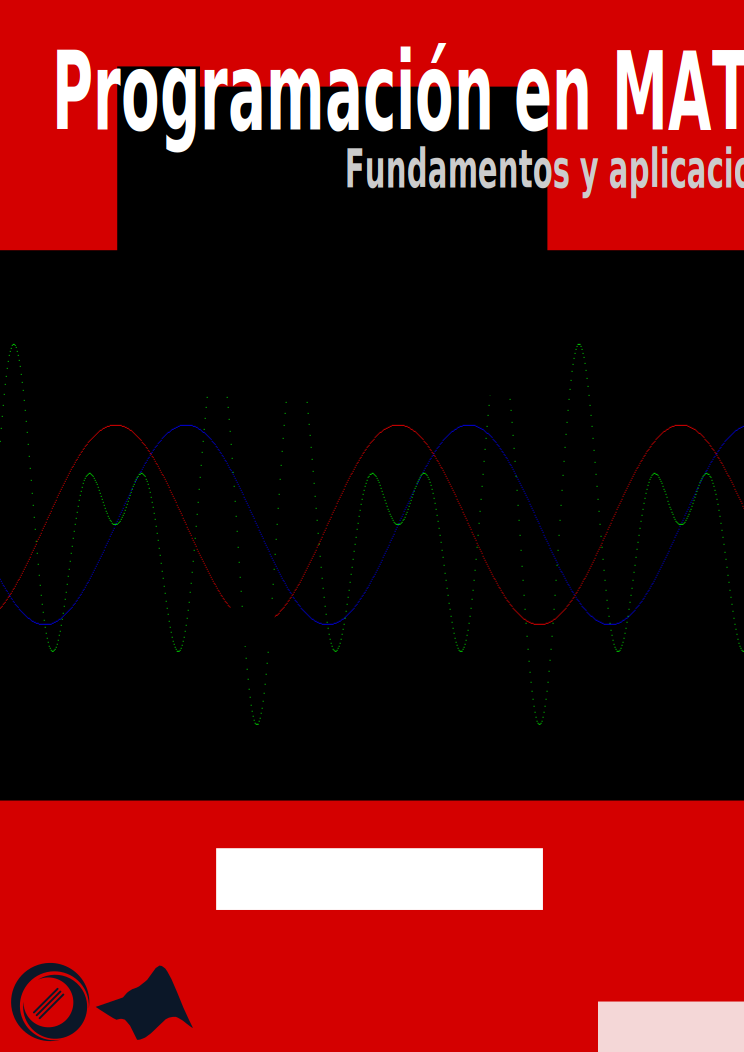
\includepdf{src/portada}
\maketitle
\tableofcontents

\makeatletter
\def\thickhrulefill{\leavevmode \leaders \hrule height 1ex \hfill \kern \z@}
\def\@makechapterhead#1{%
  \reset@font
  \parindent \z@ 
  \vspace*{15\p@}%
  \hbox{%
    \vbox{\hsize=3cm
      \begin{tabular}{c}
        \scshape \strut \@chapapp{} \\
        \fbox{%
          \vrule depth 10em width 0pt%
          \vrule height 0pt depth 0pt width 2ex%
          {\color{ccap} \fontsize{45}{2} \bfseries \strut  \thechapter}%
          \vrule height 0pt depth 0pt width 2ex%
          }
      \end{tabular}%
      }%
    \vbox{%
      \advance\hsize by -2cm
      \hrule\par
      \vskip 6pt%
      \hspace{1em}%
      \LARGE \bfseries #1
      }%
    }%
  \vskip 100\p@
}

\def\@makeschapterhead#1{%
  \reset@font
  \parindent \z@ 
  \vspace*{10\p@}%
 \hbox{%
    \vbox{\hsize=3cm
      \begin{tabular}{c}
        \scshape \strut \vphantom{\@chapapp{}} \hphantom{\@chapapp{}} \\
        \fbox{%
          \vrule depth 5em width 0pt%
          \vrule height 0pt depth 0pt width 1ex%
          {\LARGE \bfseries \strut \hphantom{\thechapter}}%
          \vrule height 10pt depth 0pt width 1ex%
          }
      \end{tabular}%
      }%
    \vbox{%
      \advance\hsize by -2cm    
      \hrule\par
      \vskip 8pt%
      \hspace{1em}%
      \LARGE \bfseries #1
      }%
    }%
  \vskip 100\p@
}

\chapter*{Acerca de...}

\section*{El libro...}

\textbf{Programación en MATLAB, fundamentos y aplicaciones} forma parte del proyecto LAB DLS, cuyo objetivo es
proporcionar herramientas a los usuarios hispanohablantes de MATLAB. %, mediante un blog y un canal de YouTube.\\

El libro consta, por ahora, de 10 capítulos en los cuales se abordan los temas básicos de la programación
en MATLAB y algunas de sus aplicaciones. Los capítulos son:\\

\begin{enumerate}
\item Fundamentos del lenguaje
\item Vectores y matrices
\item Arreglos de celdas, estructuras y cadenas de caracteres
\item Gráficas
\item Exportar e importar variables y datos
\item Matemáticas con MATLAB
\item Procesamiento de imágenes
\item Interfaces gráficas de usuario
\item Programación orientada a objetos
\item Recomendaciones generales
\end{enumerate}

El capítulo 1 abarca los temas introductorios al lenguaje, tales como el uso del entorno de desarrollo, los tipos
de datos y operadores, sentencias de control, ficheros de comandos y funciones.\\

El capítulo 2 proporciona información más detallada acerca de los vectores y matrices, cuya importancia es vital 
para sacar el máximo provecho del lenguaje, dado que es ahí donde reside la popularidad que se ha ganado.\\

El capítulo 3 está destinado a tratar otros tipos de datos más avanzados, pero que de igual forma juegan un
papel muy importante en el aprendizaje. Las cadenas de caracteres se incluyeron en este capítulo con la finalidad
de hacerlas más visibles, dado que muchas veces se tiende a subestimar en este tipo de lenguajes.\\

El capítulo 4 trata un tema muy importante como son las gráficas, en dos y tres dimensiones. Se ofrecen temas
que permiten \textit{estilizar} las gráficas y cómo exportarlas en diversos formatos.\\

El capítulo 5 se ha orientado a las diversas formas de interactuar con datos contenidos en formatos de aplicaciones 
externas, así como el manejo de las variables creadas durante una sesión de MATLAB, y claro, la manipulación de
archivos y directorios utilizando funciones nativas de MATLAB.\\

Los capítulos 6 y 7 muestran algunas aplicaciones de MATLAB en la solución de problemas comunes en matemáticas 
universitarias y procesamiento digital de imágenes, respectivamente.\\

El capítulo 8 es una introducción al desarrollo de interfaces gráficas de usuario en MATLAB, y por tanto se 
abarcan las cuestiones esenciales. Si necesita una mayor referencia en este tema, puede consultar el blog del
proyecto MATLAB TYP, se está trabajando en un texto orientado a este aspecto (Título: Desarrollo de GUIs en MATLAB) 
y se espera que a finales de 2015 esté disponible una versión inicial.\\

El capítulo 9 aborda un tema que generalmente se omite en la mayoría de los libros de esta especie: la programación
orientada a objetos (POO). Se exponen los conceptos básicos de este paradigma de programación, la sintaxis correspondiente 
al lenguaje, la organización de ficheros de clases y el manejo de objetos.\\

El capítulo 10 incluye una serie de recomendaciones que le permitirán al programador en MATLAB el desarrollo de
aplicaciones mejor documentadas, legibles y optimizadas.

\section*{La licencia...}

Este texto se distribuye bajo licencia Creative Commons BY-NC-ND 2.5 MX.\\

En resumen: usted es libre de copiar, compartir y/o distribuir este contenido, siempre y cuando se 
atribuyan los créditos correspondientes al autor del mismo y que no se haga uso de este con fines
comerciales.\\

Para una descripción más detallada de la licencia puede visitar: \url{http://creativecommons.org/licenses/by-nc-nd/2.5/mx/}

% \section*{La tipografía utilizada...}

% \subsection*{Texto}

% El texto ordinario está escrito en fuente tipo [tipo] y tamaño [tam], este parrafo es un ejemplo del mismo.

% \subsection*{Código MATLAB}

% El código MATLAB ha sido resaltado con la finalidad de hacer más legible el texto, por ejemplo:

% \begin{verbatim}	
% 	[x,y]=meshgrid(0:0.1:10);
% 	z = sin(x) + cos(y);
% 	surf(x,y,z);
% 	colormap(hot);
% \end{verbatim}

% \subsection*{Tips de programación}

% Los tips de programación incluyen información que le puede ser útil al usuario al momento de escribir código
% en MATLAB, se distingue del texto ordinario mediante un recuadro como el siguiente:

% \begin{tcolorbox}[title=Tip]
% Bla bla bla bla
% \end{tcolorbox}%


\section*{El autor...}

Ingeniero Mecánico, egresado del Instituto Tecnológico de Tuxtla Gutiérrez en el Sureste de la República
Mexicana y actualmente estudiante de posgrado en el Instituto Tecnológico de Celaya. Programador en 
Python, MATLAB, Java y C/C++.\\

\textit{Pedro Jorge De Los Santos}\\
\textit{delossantosmfq@gmail.com}\\

\href{https://labdls.blogspot.mx}{
\includegraphics[scale=0.1]{src/blogger_logo.png}}
\href{https://www.youtube.com/user/lab2dls}{
\includegraphics[scale=0.1]{src/youtube_logo.png}}
\href{https://github.com/JorgeDeLosSantos}{
\includegraphics[scale=0.08]{src/github_logo.png}}
\href{https://www.linkedin.com/in/pjdlsl}{
\includegraphics[scale=0.1]{src/linkedin_logo.png}}
\href{https://plus.google.com/u/0/+pjdelossantos}{
\includegraphics[scale=0.1]{src/google_logo.png}}



% Image Download from: https://pixabay.com/en/tiger-animal-relaxation-rest-look-1092497/
\chapter{Fundamentos del lenguaje}

\section{¿Qué es MATLAB?}

MATLAB es un lenguaje de programación de alto nivel y entorno de desarrollo interactivo, utilizado 
para numerosas aplicaciones de carácter técnico y científicas. MATLAB permite realizar adquisición 
y análisis de datos, desarrollo de algoritmos computacionales, creación y simulación de modelos físicos 
y la visualización gráfica de procesos determinados.  Entre los campos de uso de MATLAB se incluyen 
el procesamiento digital de señales,  audio, imágenes y vídeo, sistemas de control, finanzas 
computacionales, biología computacional, redes neuronales, etc.\\

\textit{Características del lenguaje:}

\begin{itemize}
\item Interpretado: Esta característica le convierte en un lenguaje no muy apto para aplicaciones donde la rapidez de ejecución sea crítica, pero esto mismo facilita la depuración de errores y permite un tiempo de desarrollo reducido en comparación a los lenguajes compilados tradicionales como C/C++.

\item Tipado dinámico: No es necesario declarar el tipo de variable a utilizar, MATLAB reconoce de forma automática el tipo de dato con el que trabajará, aunque claro que es posible declarar un tipo de dato de forma explícita utilizando las funciones de conversión adecuadas.

\item Multiplataforma: MATLAB está disponible para las plataformas más comunes: Unix, Windows, GNU/Linux y Mac OS.

\item Multiparadigma: Soporta programación imperativa, funcional y orientada a objetos.
\end{itemize}


\section{Descripción del entorno de desarrollo}

El entorno de MATLAB mostrado en la figura \ref{f1} pertenece a la versión 2012b, si dispone de otra versión 
quizá encontrará cambios significativos en la interfaz, pero los componentes más importantes permanecen invariables.\\

Como puede observarse en la figura \ref{f1}, se distinguen cuatro componentes en el escritorio del entorno MATLAB, 
los cuáles son:\\

\textbf{Command Window}\\

Ventana de comandos interactiva en la cual deberán introducirse las instrucciones de MATLAB, el prompt \texttt{$>>$} 
le indica que está listo para recibir instrucciones.\\

\begin{informacion}{¿Qué es el prompt?}
En la jerga informática, se denomina prompt al símbolo o caracter que aparece 
en una terminal o consola, cuando esta se encuentra en disposición de aceptar un comando de entrada.
\end{informacion}

\textbf{Current Folder}\\

Carpeta en la que se está situado, y en la que MATLAB buscará y guardará (por defecto) los archivos 
generados durante la sesión.\\

\textbf{Workspace}\\

Ventana que muestra las variables creadas por el usuario durante la sesión, indicando el nombre, valor 
y tipo de la misma.\\

\textbf{Command History}\\

Permite buscar comandos introducidos con anterioridad en la ventana de comandos y ejecutarlos nuevamente 
o copiarlos.\\

\begin{center}
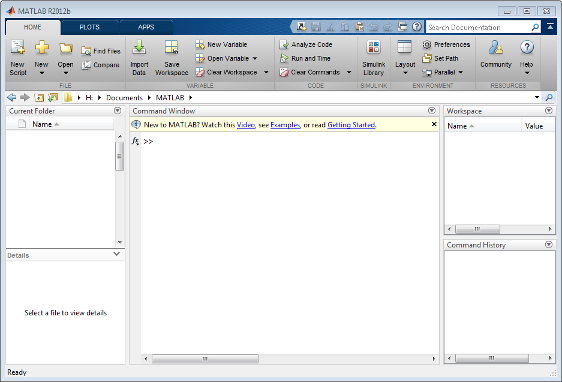
\includegraphics[scale=0.8]{src/ch1/img_1_1.png}
\captionof{figure}{Interfaz de MATLAB R2012b}
\label{f1}
\end{center}

\section{Comandos básicos y generalidades}

\subsection{Consultar ayuda de MATLAB}

Uno de los puntos fuertes de MATLAB es la extensa documentación que viene adjunta al software, la cual 
contiene múltiples ejemplos y recomendaciones para la mayoría de las funciones. Puede acceder a la ayuda 
ubicando el ícono característico de ayuda, o bien tecleando la instrucción doc en la línea de comandos.\\

Si requiere una referencia rápida acerca de un comando o función puede utilizar el comando \texttt{help} 
seguido por el nombre la función a consultar, lo anterior le mostrará en la ventana de comandos una descripción 
breve referente a la función consultada, por ejemplo la siguiente línea le permite consultar ayuda 
rápida acerca del  comando \texttt{clc}:

\begin{verbatim}
>> help clc
	clc    Clear command window.
	clc clears the command window and homes the cursor.
	See also home.
	Reference page in Help browser
	doc clc
\end{verbatim}

\subsection{Limpiar ventana de comandos y variables del workspace}

Generalmente se considera una buena práctica de programación en MATLAB iniciar los programas con 
instrucciones de limpiar la consola (Command Window) y borrar las variables de la memoria. Lo anterior 
se logra utilizando las instrucciones \texttt{clc} para limpiar la ventana de comandos y \texttt{clear} 
para borrar las variables del workspace. Suele acompañarse a la instrucción \texttt{clear} con el argumento 
adicional \texttt{all}, que permite borrar incluso variables globales, es decir 
conjuntamente: \texttt{clear all.}

\subsection{Líneas de comentarios}

Los comentarios de una sola línea en MATLAB deben comenzar  con el símbolo de porcentaje \%, todo 
aquello escrito después de este símbolo será ignorado por el intérprete y reconocido como comentario, 
asignándosele un color verde característico de forma automática.

\begin{verbatim}
% Esto es un comentario en MATLAB
\end{verbatim}

Para hacer bloques de comentarios MATLAB dispone de una sintaxis específica que se muestra enseguida:

\begin{verbatim}
	%{
	Esto es un comentario de múltiples
	líneas en MATLAB, delimitado por 
	llaves conjuntas con el signo % 
	%}
\end{verbatim}

\subsection{Valores especiales}

En la siguiente tabla se resumen algunos valores especiales devueltos por funciones predefinidas en MATLAB:

\begin{table}[h!]
\centering
{\rowcolors{1}{}{gray!20}
\begin{tabular}{p{3cm} p{12cm}} \hline
\rowcolor{header_table_color} \Centering\bfseries Función & \Centering\bfseries Descripción \\
\texttt{ans} & Guarda el ultimo valor no asignado a una variable \\
\texttt{eps} & Tolerancia que MATLAB soporta en los cálculos \\
\texttt{intmax} & Máximo valor entero que puede utilizarse \\
\texttt{intmin} & Mínimo valor entero que puede utilizarse \\
\texttt{realmax}  & Valor de coma flotante máximo que puede representarse \\
\texttt{realmin} & Valor de coma flotante mínimo que puede representarse \\
\texttt{pi} & Constante matemática (3.14159265…) \\
\texttt{inf} & Valor asignado a un número demasiado grande respecto a la
capacidad de cálculo del software. \\
\texttt{NaN} & Iniciales de “Not a Number”, tal cual traducción literal hace
referencia a un valor numérico inválido. \\
\texttt{computer} & Devuelve el tipo de computadora que se está utilizando\\
\texttt{version} & Devuelve la versión de MATLAB \\
\hline
\end{tabular}
\caption{Valores especiales}
\end{table}

\section{Tipos de datos y operadores}

Los tipos de datos más comunes en MATLAB son los siguientes:

\begin{itemize}
\item logical  (tipo booleano o lógico)
\item char (cadenas de caracteres)
\item numeric (datos tipo numérico)
\begin{itemize}
   \item int8, int16, int32, int64 (tipos entero)
   \item uint8, uint16, uint32, uint64  (enteros sin signo)
   \item single (flotantes de precisión simple)
   \item double  (flotantes de precisión doble)
\end{itemize}
\item cell (arreglos de celdas)
\item struct (estructuras)
\end{itemize}

\subsection{Tipo logical}

Las variables de tipo lógico permiten, evidentemente, dos valores, que pueden ser true o false (1 y 0 lógicos).
Una forma de declarar una variable de tipo lógico sería:

\begin{verbatim}
	>> a = true
	a =
	     1
\end{verbatim}
	     
Otra manera que resulta en lo mismo es la siguiente:

\begin{verbatim}
	>> a=logical(1)
	a =
	     1
\end{verbatim}

Las líneas anteriores crean una variable \texttt{a} de tipo lógico con un valor true (1 lógico).


\subsection{Tipo char}

Son cadenas de caracteres, que pueden contener valores alfanuméricos e incluso símbolos especiales. 
Para declararlas no hace falta especificar que son variables tipo char, dado que MATLAB es de tipado 
dinámico y reconoce como tal aquellas cuyo valor asignado se encuentre delimitado por comillas simples, 
un ejemplo muy clásico es el siguiente:

\begin{verbatim}
	>> txt = 'Hola Mundo'
	txt =
	Hola Mundo
\end{verbatim}


\subsection{Tipo numeric}

Normalmente cuando en MATLAB tecleamos un valor numérico o bien lo asignamos a una determinada variable, 
esta será de tipo double, a menos que se haga una conversión explicita a otro tipo de dato. Por ejemplo, 
si insertamos en MATLAB lo siguiente:

\begin{verbatim}
	>> num = 10
	num =
	    10
\end{verbatim}

Y posteriormente tecleamos la instrucción `whos` para verificar el tipo o clase de dicha variable:

\begin{verbatim}
	>> whos
	  Name      Size            Bytes  Class     Attributes
	  num       1x1                 8  double   
\end{verbatim}

Si se requiere utilizar un dato de tipo entero habrá de realizarse la conversión como sigue:

\begin{verbatim}
	>> numInt = int8(23)
	numInt =
	   23
	>> whos
	  Name        Size            Bytes  Class    Attributes
	  numInt      1x1                 1  int8               
\end{verbatim}

\subsection{Tipo cell}

Un cell array es un tipo de dato característico del lenguaje MATLAB que consiste en un arreglo 
multidimensional de celdas que pueden contener cualquier tipo de dato, inclusive otro cell array. 
Un ejemplo muy sencillo de cell array se muestra enseguida:

\begin{verbatim}
	>> C={10,'MATLAB','5',[1 1]}
	C = 
	    [10]    'MATLAB'    '5'    [1x2 double]
\end{verbatim}

\subsection{Tipo struct}

Las estructuras son arreglos de datos que, de forma similar a los cell arrays, pueden almacenar 
variables de diversos tipos. Para la organización de los datos se utilizan campos que pueden 
contener sólo un tipo de dato. A continuación se muestra un ejemplo de cómo crear una estructura:

\begin{verbatim}
	>> Alumno.Nombre='Jorge';
	>> Alumno.Apellido='De Los Santos';
	>> Alumno.Cursos={'Programación','Cálculo','Métodos Numéricos'};
	>> Alumno.Notas=[10 9 10];
	>> Alumno
	Alumno = 
	      Nombre: 'Jorge'
	    Apellido: 'De Los Santos'
	      Cursos: {'Programación'  'Cálculo'  'Métodos Numéricos'}
	       Notas: [10 9 10]
\end{verbatim}


En el capítulo 3 se tratan con más detenimiento las estructuras y su utilidad en la programación en MATLAB.


\subsection{Referencias de función (function handle)}

Las function handle son referencias asociadas a una función nativa de MATLAB o bien a una función 
anónima creada por el usuario.\\

El siguiente ejemplo muestra la creación de una función anónima y su posterior uso mediante su referencia:

\begin{verbatim}
	>> f=@(x) x+cos(x)
	f = 
	    @(x)x+cos(x)
	>> whos
	  Name      Size            Bytes  Class              Attributes
	  f         1x1                32  function_handle              
	>> fzero(f,0) % Raíz de la función 
	ans =
	   -0.7391
	>> f(pi/2) % Evaluando función en un punto
	ans =
	    1.5708
\end{verbatim}


\subsection{Identificar tipos de datos}

Para identificar tipos de datos en MATLAB se cuentan con diversos comandos que nos facilitan esta tarea. 
El comando whos nos proporciona información acerca de las variables existentes en el workspace, tales 
como el nombre, tamaño y tipo. A manera de ejemplo crearemos las siguientes variables e introducimos la 
instrucción whos para verificar el tipo de información que nos imprime en la consola:

\begin{verbatim}
 	>> n=10;
	>> val=false;
	>> s='MATLAB';
	>> C={1,2,3};
	>> ST.Nombre='Anna';
	>> whos
	  Name      Size            Bytes  Class      Attributes
	  C         1x3               360  cell                 
	  ST        1x1               184  struct               
	  n         1x1                 8  double               
	  s         1x6                12  char                 
	  val       1x1                 1  logical      
 \end{verbatim} 


Además del comando \texttt{whos}, puede utilizarse la función \texttt{class} para determinar el tipo de dato de una 
variable pasada como argumento, por ejemplo:

\begin{verbatim}
	>> a=3;
	>> class(a)
	ans =
	double
\end{verbatim}

\subsection{Conversiones entre tipos de datos}

Las conversiones entre tipos de datos son muy utilizadas en la programación en cualquier lenguaje, 
puesto que permiten controlar la precisión de los cálculos, mejorar la presentación de los datos o 
bien evitar errores en la ejecución.

\subsubsection{Entre tipos numéricos}

Cuando se crea una variable de tipo numérico en MATLAB por defecto será de tipo double, por ejemplo, 
creamos una variable llamada num:

\begin{verbatim}
	>> num=2;
	>> class(num)
	ans =
	double
\end{verbatim}

Las conversiones entre tipos numéricos son de sintaxis muy sencilla, solo habrá que especificar el 
tipo de dato al cual se convertirá, siendo permitidos los especificados en la tabla siguiente:\\

\begin{table}[h!]
\centering
{\rowcolors{1}{}{gray!20}
\begin{tabular}{p{5cm} p{5cm} p{5cm}}
\rowcolor{header_table_color} \Centering\bfseries Tipo de dato & \Centering\bfseries Sintaxis de conversión & 
\Centering\bfseries Rango \\
Precisión doble & double(num) & 2.2251e-308 a 1.7977e+308 \\
Precisión simple & single(num) & 1.1755e-38 a 3.4028e+38 \\
Entero de 8 bits & int8(num) & -128 a 127 \\
Entero de 16 bits & int16(num) & -32768 a 32767 \\
Entero de 32 bits & int32(num) & -231 a 231-1 \\
Entero de 64 bits & int64(num) & -263 a 263-1 \\
Entero sin signo de 8 bits & uint8(num) & 0 a 255 \\
Entero sin signo de 16 bits & uint16(num) & 0 a 65535 \\
Entero sin signo de 32 bits & uint32(num) & 0 a 4294967295 \\
Entero sin signo de 64 bits & uint64(num) & 0 a 18446744073709551615 \\
\end{tabular}
\caption{Conversiones entre tipos numéricos}
\end{table}

Así, podemos convertir la variable num, creada con anterioridad, a otro tipo de dato numérico, por 
ejemplo a un entero de 8 bits:

\begin{verbatim}
	>> num=int8(num);
	>> class(num)
	ans =
	int8
\end{verbatim}

Es necesario poner especial atención en los rangos que pueden manipularse con cada tipo numérico, 
debido a que por ejemplo si se realiza la siguiente conversión:

\begin{verbatim}
	>> num=int8(653)
	num =
	  127
\end{verbatim}

El valor que ha sido pasado como argumento de conversión excede el rango para un entero de 8 bits, 
por lo cual simplemente se le asigna el máximo valor permitido para una variable de este tipo.\\

Si requiere verificar por usted mismo los valores máximos y mínimos permitidos para cada tipo de dato, 
puede usar las funciones \texttt{realmin} y \texttt{realmax} para los tipos de coma flotante, y las 
correspondientes \texttt{intmin} e \texttt{intmax} para tipos enteros.

\subsubsection{De string a tipo numérico}

Para este tipo de conversiones MATLAB dispone de la funciones \texttt{str2double} y \texttt{str2num}, 
en algunos casos no notará la diferencia en los resultados, salvo en la rapidez de ejecución. Pese a lo 
anterior, es necesario tomar en cuenta cómo trabaja cada función y cual le resulta de utilidad; 
con \texttt{str2double} se convierte una variable tipo string en un valor de tipo double, 
la función \texttt{str2num} también realiza conversión a tipo double pero además realiza conversiones 
a otros tipos de datos numéricos si se especifica de manera explícita, de hecho esta tiene una 
funcionalidad muy similar a la de la función \texttt{eval}. Los siguientes ejemplos muestran las 
diferencias y utilidades de las funciones descritas.


\begin{verbatim}
	>> a=str2double('1237')
	a =
	        1237
	>> b=str2num('1237')
	b =
	        1237
	>> whos
	  Name      Size            Bytes  Class     Attributes
	  a         1x1                 8  double              
	  b         1x1                 8  double     
\end{verbatim}


\subsection{Operadores aritméticos, relacionales y lógicos}

En la siguiente tabla se resumen los operadores más importantes en MATLAB.

\begin{table}[h!]
\centering
{\rowcolors{1}{}{gray!20}
\begin{tabular}{p{3cm} p{9cm}}
\rowcolor{header_table_color} \Centering\bfseries Operador  & \Centering\bfseries Descripción \\
\multicolumn{2}{c}{\bfseries Operadores aritméticos} \\
+ & Operador  suma \\
- & Operador resta \\
* & Operador multiplicación (escalares) \\
/ & Operador división \\
./ & División elemento a elemento (matrices) \\
.* & Multiplicación elemento a elemento (matrices) \\
\multicolumn{2}{c}{\bfseries Operadores lógicos} \\
\& & Operador lógico and \\
$|$ & Operador lógico or \\
$\sim$ & Operador lógico not \\
\multicolumn{2}{c}{\bfseries Operadores relacionales} \\
== & Igual a  \\
$<$ & Menor que \\
$>$ & Mayor que \\
$<$= & Menor o igual que \\
$>$= & Mayor o igual que \\
$\sim =$ & Diferente de \\
\end{tabular}
\caption{Conversiones entre tipos numéricos}
\end{table}


\section{Un mini tutorial de introducción}

Una vez conocidos los tipos de datos y los operadores, podemos comenzar con una breve introducción 
al uso de MATLAB como una poderosa calculadora muy fácil de utilizar.\\

Como se ha descrito en secciones anteriores, el command window o ventana de comandos es la parte 
del entorno MATLAB que nos permite interactuar de forma dinámica, si tecleamos una instrucción 
automáticamente nos devolverá un resultado y se crearán variables en las cuales se almacenen 
los diversos valores de salida. Por ejemplo, vamos a teclear una simple suma aritmética:

\begin{verbatim}
	>> 3+2
	ans =
	     5
\end{verbatim}

Puede verificar que en el workspace ahora aparece una variable llamada \texttt{ans} con valor de 5, 
en \texttt{ans} se guarda por defecto el último resultado no asignado a una variable, podríamos asignar 
el resultado de la suma a una variable específica:

\begin{verbatim}
	>> suma=3+2
	suma =
	     5
\end{verbatim}

Podemos también asignar valores a determinadas variables y enseguida utilizarlas para ejecutar 
alguna operación, por ejemplo:

\begin{verbatim}
	>> a=5;
	>> b=7;
	>> a*b
	ans =
	    35
	>> a-b
	ans =
	    -2
	>> a/b
	ans =
	    0.7143
\end{verbatim}

Note que el colocar un punto y coma (;) al final de una instrucción evita que se muestre un resultado de salida, 
lo cual no afecta en el almacenamiento de los valores correspondientes, pero podría resultar de mucha ayuda al 
momento de seleccionar los valores que se quieren mostrar en la ventana de comandos.\\

MATLAB también tiene disponible diversas funciones matemáticas predefinidas, que pueden ser aplicadas 
sobre un número o sobre una matriz o arreglo de números. Algunas funciones trigonométricas:

\begin{verbatim}
	>> sin(pi/2)
	ans =
	     1
	>> cos(pi/4)
	ans =
	    0.7071
	>> tan(pi/3)
	ans =
	    1.7321
\end{verbatim}

Note que el valor de la constante $\pi$ está predefinida en MATLAB mediante la cadena \texttt{pi}:

\begin{verbatim}
>> pi
ans =
    3.1416
\end{verbatim}

MATLAB devuelve un valor de 3.1416, lo cual es un valor \textit{redondeado} de $\pi$, pero esto 
es cuestión solamente de la representación, normalmente se utiliza el formato short (4 dígitos después
del punto decimal) para la representación de valores numéricos, internamente MATLAB utiliza más 
digitos para \textit{manejar} y operar con el valor de $\pi$. Si queremos obtener más digitos en 
la salida por consola podemos cambiar el formato de salida:

\begin{verbatim}
>> format long
>> pi
ans =
   3.141592653589793
\end{verbatim}

El formato largo permite representar una cantidad con 16 decimales. Incluso es posible \textit{forzar} 
a que se muestre una representación en forma racional:

\begin{verbatim}
>> format rat
>> pi
ans =
     355/113   
>> 0.1+0.123
ans =
     223/1000  
>> 0.125
ans =
       1/8
\end{verbatim}

Se puede crear una lista o arreglo de valores numéricos encerrando estos entre corchetes, 
y separando cada elemento por comas o espacios.

\begin{verbatim}
>> A=[5,8,10,2,7]
A =
     5     8    10     2     7
>> B=[3 7 1 0 -2]
B =
     3     7     1     0    -2
\end{verbatim}

Se puede obtener el valor máximo y mínimo de un arreglo numérico utilizando las funciones \texttt{max} y 
\texttt{min} respectivamente.

\begin{verbatim}
>> max(A)
ans =
    10
>> min(A)
ans =
     2
\end{verbatim}

También podemos calcular el promedio de los valores utilizando la función \texttt{mean}:

\begin{verbatim}
>> mean(A)
ans =
    6.4000
\end{verbatim}

Obtener la cantidad de elementos que componen lista con \texttt{length} o \texttt{numel}:

\begin{verbatim}
>> length(A)
ans =
     5
>> numel(A)
ans =
     5
\end{verbatim}


\section{Ficheros de comandos}

Los ficheros de comandos, conocidos también como \textit{scripts}, son archivos de texto sin formato 
(ASCII) con la extensión característica de los archivos de MATLAB (*.m), se utilizan para 
almacenar una serie de comandos o instrucciones que se ejecutan sucesivamente y que habrán 
de realizar una tarea específica. Los scripts de MATLAB pueden editarse utilizando cualquier 
editor de texto sin formato (Bloc de Notas, Notepad++, Sublime Text, etc…), aunque es más 
recomendable utilizar el editor de MATLAB, puesto que proporciona herramientas que facilitan 
la corrección de errores, el control sobre la ejecución del código y la capacidad de 
autocompletado y sugerencias cuando se utilizan funciones nativas de MATLAB.\\

Para crear un nuevo script puede pulsar la combinación \textbf{Ctrl + N} (bajo SO Windows), o buscar 
en la interfaz de MATLAB la opción New y enseguida seleccionar Script; si prefiere hacerlo 
desde la ventana de comandos puede introducir el comando edit que le abrirá un nuevo script.\\

Para guardar un fichero de comandos utilice la opción \textbf{Save} de la barra de herramientas  o 
bien mediante la combinación de teclas \textbf{Ctrl + S} en Windows. Debe tomarse en cuenta que 
al guardar un script se le proporcione un nombre que no entre en conflicto con las funciones 
nativas de MATLAB o las palabras reservadas del lenguaje. Algunas recomendaciones que deben 
seguirse para nombrar un script son:

\begin{itemize}
\item El nombre deberá contener sólo letras, números o guiones bajos.
\item No deberá comenzar con un carácter diferente a una letra (Por ejemplo: 102metodo.m, es un nombre inválido dado que comienza con un número).
\item Evite utilizar nombres de funciones nativas de MATLAB o palabras reservadas del lenguaje que podrían ocasionar conflictos.
\end{itemize}






\section{Entradas y salidas en el Command Window}

En la sección 1.2 se describió al Command Window (ventana de comandos) y se hizo referencia a este 
como la parte del escritorio de MATLAB que permite interactuar tecleando instrucciones y 
devolviendo al instante un resultado. En esta sección veremos cómo utilizar funciones que 
permitan introducir y mostrar ciertos valores de manera controlada por el usuario.

\subsection{La función input}

La función input permite \textit{pedir} un valor al usuario utilizando una cadena de caracteres 
como prompt, la sintaxis es muy sencilla:

\begin{verbatim}
	var=input('Introduzca un valor: ');
\end{verbatim}

En la variable var se guarda el valor que el usuario introduzca, los valores aceptados por 
la función input pueden ser de tipo numérico, cell arrays, e inclusive tipo char. Aunque 
para introducir cadenas de texto la función input dispone de un modificador que hará que 
la entrada se evalúe como una variable tipo char o cadena de texto, la sintaxis para 
esto es la siguiente:

\begin{verbatim}
	var=input('Introduzca una cadena de texto: ', 's');
\end{verbatim}

La letra s entre comillas simples le indica a MATLAB que deberá evaluar la entrada como tipo string.

\subsection{Salida sin formato: la función disp}

La función disp muestra en pantalla el valor de una determinada variable que se pasa como 
argumento, por ejemplo:

\begin{verbatim}
	>> a=3;
	>> disp(a)
	     3
\end{verbatim}

Para el caso anterior se pasa como argumento la variable a que ha sido declarada previamente 
y simplemente se muestra el valor correspondiente a esta. Las variables a mostrar pueden ser 
de cualquier tipo, incluyendo cadenas de texto, matrices, cell arrays y estructuras, 
véanse los siguientes ejemplos:

\begin{verbatim}
	>> disp(magic(3))
	     8     1     6
	     3     5     7
	     4     9     2
	>> disp({1,0,2,-2})
	    [1]    [0]    [2]    [-2]
	>> disp('Hola Mundo')
	Hola Mundo
\end{verbatim}

Con disp también es posible mostrar enlaces a un sitio web, utilizando la sintaxis HTML para 
un enlace dentro de la función disp, por ejemplo:

\begin{verbatim}
	>> disp('<a href="http://matlab-typ.blogspot.mx">MATLAB TYP</a>');
	MATLAB TYP
\end{verbatim}

\subsection{La función fprintf}

Con fprintf es posible dar formato a la salida que se quiere imprimir en pantalla, por ejemplo, es posible
especificar el número de decimales que se mostrarán o bien si se quiere mostrar como un entero o quizá
como una cadena de texto. La sintaxis de la función fprintf es como sigue:

\begin{verbatim}
fprintf('Especificaciones de formato',a1,...,an);
\end{verbatim}

Donde las especificaciones de formato incluyen uno o más de los identificadores de un mismo tipo o
combinados que se muestran en la siguiente tabla:

\begin{table}[h!]
\centering
{\rowcolors{1}{}{gray!20}
\begin{tabular}{p{4cm} p{7cm}} \hline
\rowcolor{header_table_color} \Centering\bfseries Identificador & \Centering\bfseries Formato de salida \\
\texttt{\%d} & Tipo entero \\
\texttt{\%f} & Tipo coma flotante \\
\texttt{\%g} & Tipo coma flotante compacta. \\
\texttt{\%u} & Tipo entero sin signo \\
\texttt{\%e} & Tipo coma flotante, notación exponencial \\
\texttt{\%s} & Tipo char, cadena de texto \\
\texttt{\%c} & Tipo char, carácter a carácter.\\
\hline
\end{tabular}
\caption{Opciones de formato para \texttt{fprintf}}
\end{table}

Véase el siguiente ejemplo:

\begin{verbatim}
>> fprintf('%d',pi);
3.141593e+00>>
\end{verbatim}

Observe que se imprime el valor de $\pi$ en este caso, pero el prompt de la ventana de comandos queda situado
justo después del valor de salida en la misma línea, para evitar lo anterior puede utilizar la secuencia de
escape \n después del valor a imprimir, lo cual le indica a MATLAB que debe comenzar en una nueva
línea. Modificamos y vemos el resultado que produce:

\begin{verbatim}
>> fprintf('%d\n',pi);
3.141593e+00
\end{verbatim}

Ahora observe lo que se imprime utilizando otros identificadores:

\begin{verbatim}
>> fprintf('%f\n',pi);
3.141593
>> fprintf('%g\n',pi);
3.14159
>> fprintf('%e\n',pi);
3.141593e+00
>> fprintf('%u\n',pi);
3.141593e+00
\end{verbatim}

Para las salidas de coma flotante puede especificar el número de decimales que tendrá la salida, por ejemplo
si desea mostrar solamente dos decimales del número $\pi$:

\begin{verbatim}
>> fprintf('%.2f\n',pi);
3.14
\end{verbatim}


\section{Funciones}

\subsection{Funciones, una introducción}

Las funciones son porciones de código que por lo general aceptan argumentos o valores de 
entrada y devuelven un valor de salida. Una función es una herramienta muy útil en la 
programación, dado que permite la reutilización de código para procedimientos que así 
lo requieran, así como una facilidad significativa para mantener el código, lo cual se 
traduce en una mayor productividad.  MATLAB, de hecho, está compuesto por una multitud 
de funciones agrupadas en toolboxs, cada una de ellas pensada para resolver una 
situación concreta.\\

La estructura básica de una función contiene los siguientes elementos:

\begin{itemize}
\item La palabra reservada function
\item Los valores de salida
\item El nombre de la función
\item Los argumentos de entrada
\item Cuerpo de la función 
\end{itemize}

Para una mejor comprensión de cada uno de esos elementos, refiérase a las siguientes 
líneas de código:

\begin{verbatim}
	function res = suma(a,b)
	res = a+b;
	end
\end{verbatim}

La función anterior llamada suma, recibe como argumentos de entrada dos valores numéricos 
a y b, y devuelve un resultado guardado en res que equivale a la suma aritmética de las 
variables de entrada. Si ejecutamos la función en la ventana de comandos obtenemos 
algo similar a esto:

\begin{verbatim}
	>> s=suma(3,2)
	s =
	     5
\end{verbatim}

Si no hace una asignación el resultado devuelto se guarda en la variable \texttt{ans}.

\subsection{Verificar argumentos de entrada y salida}

Cuando se crea una función es recomendable verificar si la cantidad de argumentos de 
entrada corresponden a los soportados, o bien, si el tipo de dato que se ha introducido 
es el adecuado para proceder con el resto de la programación; MATLAB proporciona los 
comandos \texttt{nargin} y \texttt{nargout} que sirven para \textit{contar} el número de argumentos de 
entrada y salida respectivamente.\\

Utilizando como ejemplo la función suma creada con anterioridad, podemos verificar que 
el número de argumentos sean exactamente dos para poder proceder y en caso contrario 
enviar al usuario un mensaje de error en la ventana de comandos, el código implicado 
sería similar al siguiente:

\begin{verbatim}
	function res = suma(a,b)
	if nargin==2
	    res=a+b;
	else
	    error('Introduzca dos argumentos de entrada');
	end
	end
\end{verbatim}

Si ejecutamos la función pasándole solamente un argumento de entrada nos devolverá un mensaje de error:

\begin{verbatim}
	>> s=suma(7)
	Error using suma (line 5)
	Introduzca dos argumentos de entrada
\end{verbatim}

\subsection{Sub-funciones}

Las sub-funciones son funciones definidas dentro del espacio de otra función principal. 
Se utilizan como funciones auxiliares con la finalidad de hacer más legible el código y 
facilitar la depuración de errores. Enseguida se muestra el ejemplo de una sub-función:

\begin{verbatim}
	function r=isfibo(num)
	% Determina  si un  número  entero  forma  parte
	% de la sucesión de Fibonacci, devuelve un valor
	% de tipo lógico.
	ff=fibonacci(num);
	if any(ff==num)
	    r=true;
	else
	    r=false;
	end
	    function F=fibonacci(n)
	        F(1:2)=1;
	        i=3;
	        while 1
	            F=[F F(i-1)+F(i-2)];
	            if F(end) >= n,break,end;
	            i=i+1;
	        end
	    end
	end
\end{verbatim}

La función anterior isfibo determina si el entero pasado como argumento de entrada 
pertenece a la sucesión de Fibonacci, para ello utiliza como una función auxiliar a 
la sub-función fibonacci que se encarga de generar la sucesión de Fibonacci en un 
intervalo dado y guardarlo en un vector de salida. Una sub-función puede ser llamada 
solamente por la función principal que la contiene.

\subsection{Argumentos variables}

En la introducción a las funciones se ha mencionado que estas por lo general 
tienen un número específico de argumentos de entrada y salida, no obstante se 
presentan situaciones en donde  los argumentos de entrada o salida de una función 
no son fijos o bien los argumentos pueden ser demasiados de tal modo que resulte 
incómodo definirlos en la línea correspondiente. Para solucionar lo anterior MATLAB 
permite el uso de varargin y varargout como argumentos de entrada y salida 
respectivamente. Para tener una  idea más práctica de lo anterior véase el ejemplo siguiente:

\begin{matlab}
	function m=max2(varargin)
	if nargin==1
	    v=varargin{1};
	    m=v(1);
	    for i=2:length(v)
	        if v(i)>m
	            m=v(i);
	        end
	    end 
	elseif nargin==2
	    a=varargin{1};
	    b=varargin{2};
	    if a>b
	        m=a;
	    else
	        m=b;
	    end
	end
	end
\end{matlab}

La función anterior max2 emula a la función nativa  max, puede recibir como argumento 
de entrada un vector o bien dos valores escalares. Si observa el código anterior notará 
que varargin es un cell array que guarda todos los argumentos de entrada pasados a la 
función, como se verá en el capítulo 3 la manera de acceder a los elementos de un 
cell array es utilizando la sintaxis: var{k}, donde var es la variable en la que está 
almacenada el cell array y k es el k-ésimo elemento contenido en el cell array.

\subsection{Ayuda de una función}

Como parte de las buenas prácticas de programación es recomendable incluir comentarios 
dentro de una función que indiquen el propósito de esta, así como una descripción breve 
de los argumentos de entrada y salida e incluso un ejemplo concreto de la misma.\\

Por convención estos comentarios deben colocarse justamente después de la definición de 
la función y antes de todo el código restante, además de que esto servirá como referencia 
al resto de usuarios también le permitirá a MATLAB interpretarlo como las líneas de ayuda 
cuando se le solicite expresamente mediante la función help. Véase el siguiente ejemplo:

\begin{verbatim}
	function [x1,x2]=ecuad(a,b,c)
	% Resuelve una ecuación cuadrática de la forma:
	% a*x^2+b*x+c=0
	%
	% Argumentos de entrada:
	%          a  -  Coeficiente cuadrático
	%          b  -  Coeficiente lineal
	%          c  -  Coeficiente constante
	%
	% Argumentos de salida:
	%          x1,x2  - Raíces de la ecuación cuadrática 
	%
	% Ejemplo:
	%         >> [r1,r2]=ecuad(-1,2,1);
	%
	 
	x1=(1/(2*a))*(-b+sqrt(b^2-4*a*c));
	x2=(1/(2*a))*(-b-sqrt(b^2-4*a*c));
	end
\end{verbatim}

Podemos teclear help ecuad en la ventana de comandos y verificar lo que MATLAB nos 
devuelve como ayuda de la función:

\begin{verbatim}
	>> help ecuad
	  Resuelve una ecuación cuadrática de la forma:
	  a*x^2+b*x+c=0
	  Argumentos de entrada:
	           a  -  Coeficiente cuadrático
	           b  -  Coeficiente lineal
	           c  -  Coeficiente constante
	  Argumentos de salida:
	           x1,x2  - Raíces de la ecuación cuadrática 
	  Ejemplo:
	          >> [r1,r2]=ecuad(-1,2,1);
\end{verbatim}

Es común agregar a la ayuda de una función algunas referencias hacia otras funciones 
similares, para ello en los comentarios debe agregar una línea que comience con las 
palabras “SEE ALSO” (Ver también), seguidas de las funciones similares separadas por 
comas, véase el ejemplo a continuación:

\begin{verbatim}
	function [x1,x2]=ecuad(a,b,c)
	% Resuelve una ecuación cuadrática de la forma:
	% a*x^2+b*x+c=0
	%
	% Argumentos de entrada:
	%          a  -  Coeficiente cuadrático
	%          b  -  Coeficiente lineal
	%          c  -  Coeficiente constante
	%
	% Argumentos de salida:
	%          x1,x2  - Raíces de la ecuación cuadrática 
	%
	% Ejemplo:
	%         >> [r1,r2]=ecuad(-1,2,1);
	%
	% SEE ALSO roots,solve,fzero
	%
	 
	x1=(1/(2*a))*(-b+sqrt(b^2-4*a*c));
	x2=(1/(2*a))*(-b-sqrt(b^2-4*a*c));
	end
\end{verbatim}

\begin{verbatim}
	>> help ecuad
	  Resuelve una ecuación cuadrática de la forma:
	  a*x^2+b*x+c=0 
	  Argumentos de entrada:
	           a  -  Coeficiente cuadrático
	           b  -  Coeficiente lineal
	           c  -  Coeficiente constante
	  Argumentos de salida:
	           x1,x2  - Raíces de la ecuación cuadrática 
	  Ejemplo:
	          >> [r1,r2]=ecuad(-1,2,1);

	  SEE ALSO roots,solve,fzero
\end{verbatim}

\section{Bifurcaciones y bucles}

\subsection{Sentencia if-elseif-else}

La sentencia if se utiliza  como bifurcación simple por sí sola, es decir, en aquellas 
situaciones en las cuales se requiera evaluar solamente una condición, por ejemplo, 
suponga que tiene dos números a y b y necesita comprobar si son iguales y ejecutar una 
acción, para ello bastaría con una sentencia if simple:

\begin{verbatim}
	if a==b
	    disp('a es igual a b');
	end
\end{verbatim}

A  diferencia del caso anterior hay situaciones que requieren la ejecución de una acción 
cuando la condición se cumpla y de otra en caso contrario, entonces puede utilizarse 
una bifurcación doble formada por las sentencias  if-else. Retomando el ejemplo para 
la bifurcación if simple, podríamos modificarlo de tal manera que envíe también un 
mensaje (ejecute una acción) para cuando la condición no se cumple:

\begin{verbatim}
	if a==b
	    disp('a es igual a b');
	else
	    disp('a es diferente de b');
	end
\end{verbatim}

Ahora imagine que para los ejemplos anteriores  se necesita especificar si  a=b, si a>b 
o bien si a<b, lo cual implicaría tener una sentencia de selección múltiple 
if-elseif-else que permite escoger entre varias opciones, evaluándose en orden 
descendente, por ejemplo refiérase a la siguiente estructura:

\begin{verbatim}
	if cond1
	    % Instrucciones
	elseif cond2 
	    % Instrucciones
	elseif cond3
	    % Instrucciones
	    .
	    .
	    .
	elseif condN
	    % Instrucciones
	else
	    % Instrucciones
	end
\end{verbatim}

MATLAB evalúa primeramente la condición 1 contenida en la sentencia if (cond1) y en 
el caso de no cumplirse evalúa la siguiente condición de forma sucesiva (cond2, cond3, …); 
finalmente y en el caso de que ninguna de las opciones evaluadas se cumpla, se ejecuta 
la instrucción contenida en la sentencia else. A continuación se muestra el ejemplo de 
una bifurcación múltiple para la situación descrita al principio:

\begin{verbatim}
	if a==b
	    disp('a es igual que b');
	elseif a>b
	    disp('a es mayor que b');
	elseif a<b
	    disp('a es menor que b');
	end
\end{verbatim}

\subsection{Sentencia switch}

La sentencia switch es una bifurcación múltiple que permite seleccionar entre varias 
opciones o casos la acción a ejecutar. La sintaxis general es:

\begin{verbatim}
	switch var
	   case opc1
	      % Instrucciones
	   case opc2
	      % Instrucciones
	    .
	    .
	    .
	   otherwise
	      % Intrucciones
	end
\end{verbatim}

Siendo var la variable que servirá como criterio de selección. Después de la palabra 
reservada case, se coloca el valor de var para el cual se ejecutarán esas instrucciones, 
y en otherwise se insertan las instrucciones que MATLAB deberá ejecutar por defecto en 
caso de no cumplirse ninguno de los casos especificados.\\

Enseguida se muestran dos ejemplos correspondientes a la sentencia de selección switch:

\begin{verbatim}
	X=input('Inserte 0 o 1: ');
	switch X
	    case 0
	        disp('Insertó cero');
	    case 1
	        disp('Insertó uno');
	    otherwise
	        warning('Valor incorrecto, verifique');     
	end


	letra=input('Inserte una letra: ','s');
	switch letra
	    case {'a','e','i','o','u'}
	        disp('Es una vocal');
	    otherwise
	        disp('Es una consonante');
	end
\end{verbatim}


\subsection{Bucle for}

La sintaxis general de un bucle for se muestra enseguida:

\begin{verbatim}
	for i=inicio:incremento:fin
	    % Instrucciones...
	end
\end{verbatim}

El valor inicio es a partir del cual se ejecutará el ciclo, el incremento es la 
cantidad que varía en cada paso de ejecución, y el valor de final establece el 
último valor que  tomará el ciclo.\\

El siguiente código muestra un ciclo for muy básico, el cual simplemente muestra 
en consola el valor actual adquirido por la variable.

\begin{verbatim}
	for i=1:10
	    fprintf('Valor actual: %g \n',i);
	end
\end{verbatim}

Cuando no se especifica el incremento, como el caso anterior, MATLAB asume que es unitario.\\

Es posible utilizar ciclos for anidados, por ejemplo para cuando se requiere 
recorrer una matriz en sus dos dimensiones y ejecutar operaciones elemento 
por elemento. Véase el siguiente ejemplo:

\begin{verbatim}
	A=round(rand(5)*10);
	for i=1:5
	    for j=1:5
	        disp(A(i,j));
	    end
	end
\end{verbatim}


\subsection{Bucle while}

El bucle while se utiliza, por lo general, cuando no se tiene un rango definido 
sobre el cual se realice la ejecución del ciclo o bien cuando la terminación del 
mismo viene dada por una condición. La sintaxis más común es:

\begin{verbatim}
	while cond
	    % Instrucciones
	    % ...
	    % ...
	    % ...
	end
\end{verbatim}

Donde \texttt{cond} es la condición que determina la finalización de ejecución.\\

Enseguida se muestra un ejemplo muy básico que muestra en pantalla el valor 
de una variable utilizada como referencia:

\begin{verbatim}
	k=1;
	while k<10
	    disp(k);
	    k=k+1;
	end
\end{verbatim}

Lo anterior muestra en consola el valor de k mientras esta sea menor a 10, es decir 
muestra todos los valores enteros en el intervalo [1  9], es importante notar que 
la variable k debe incrementarse en cada ciclo para que en un momento determinado 
la condición de finalización se cumpla, de lo contrario se convertiría en un bucle infinito.\\

Ahora, veamos un ejemplo más práctico. La aproximación de una raíz cuadrada por 
el método babilónico implica realizar n iteraciones mediante la siguiente expresión:

$$r_n(x) = \frac{1}{2}(\frac{x}{r_{n-1}}+r_{n-1})$$

Donde x es el número del cual se calcula la raíz cuadrada. A continuación se muestra 
el código implementado en MATLAB utilizando un bucle \texttt{while}:

\begin{verbatim}
	x=input('Introduzca un número positivo: ');
	r=x;
	ra=0;
	while ra~=r
	    ra=r;
	    r=(1/2)*(x/r+r);
	end
	fprintf('\nRaíz cuadrada de %g = %g\n\n',x,r);
\end{verbatim}

Como se observa, en la variable ra se guarda la raíz aproximada calculada en una 
iteración anterior, de manera que esta sirva como comparación respecto a la nueva 
raíz calculada, el bucle termina cuando la diferencia entre el valor actual y el 
anterior es inferior a la tolerancia numérica (eps) soportada por MATLAB y por 
ende pasan a considerarse como valores iguales.

\begin{informacion}{El bucle while \& if-break}
Es común utilizar el ciclo while poniendo un valor verdadero como condición, y 
usar la sentencia combinada \texttt{if-break} como punto de parada, por ejemplo:

\begin{verbatim}
while true
    a = randi(10);
    if a>5
        break;
    end
end
\end{verbatim}

\end{informacion}


\section{Fecha y hora}

Primeramente es importante mencionar que MATLAB maneja tres formatos de fechas 
y hora, a saber:

\begin{itemize}
\item Un vector de seis elementos los cuales son: [año, mes, día, hora, minuto, segundo].
\item Un valor escalar de coma flotante (tipo double), en el cual la parte entera representa la cantidad de días que han transcurrido desde el año cero (calendario gregoriano) y la parte decimal representa la fracción del día trascurrido.
\item Una cadena de texto con la forma \texttt{'dd-mmm-aaa HH:MM:SS'}.
\end{itemize}

Para obtener la fecha actual MATLAB proporciona el comando now:

\begin{verbatim}
	>> now
	ans =
	   7.3575e+05
\end{verbatim}

Lo anterior podría resultar útil para efectos de cálculo pero no es tan significativo 
para el usuario que está acostumbrado a visualizar la fecha y hora mediante los formatos 
convencionales; podemos convertir el valor numérico anterior a una cadena de texto que 
nos proporcione mayor información a primer vista, para ello se utiliza la función 
datestr como sigue:

\begin{verbatim}
	>> datestr(now)
	ans =
	03-Jun-2014 17:09:36
\end{verbatim}

Además de las anteriores MATLAB dispone de las funciones datevec y clock, la primera 
convierte una determinada fecha pasada como argumento en formato string o numérico a 
un vector de seis elementos como se describió anteriormente, y clock devuelve la fecha 
y hora actual tal como la hace now pero  como un vector de seis elementos.



% ==========================================================================================================

\begin{ejemplo}{Ejemplo 1.1}
El número de Reynolds es un parámetro adimensional utilizado en mecánica de fluidos para caracterizar el
movimiento de un fluido, usualmente se define como:

$$ Re=\frac{vD}{\nu} $$

Donde v es la velocidad del fluido, D el diámetro de la tubería a través de la cual circula el fluido y $\nu$ la
viscosidad cinemática. La teoría subyacente del número de Reynolds se establece conforme a varias
características propias y externas al fluido, pero en este caso vamos a limitarlo al flujo interno en tuberías
circulares; siendo así, el número de Reynolds permite caracterizar si un flujo es laminar o turbulento
dependiendo de ciertos intervalos establecidos de manera experimental, enseguida se muestran los intervalos
de valores y el tipo de flujo en cada caso:\\

Re $<$ 2100  \textit{Flujo turbulento}\\
2100 $\leq$ Re $\leq$ 3000   \textit{Flujo transitorio}\\
Re $>$ 3000    \textit{Flujo turbulento}\\

Basado en lo anterior, escriba un programa cuyos valores de entrada sean la velocidad del fluido, el diámetro
de la tubería y la viscosidad cinemática, y que devuelva como variable de salida el tipo de flujo.
\end{ejemplo}
% ==========================================================================================================




\section*{Problemas}

\textbf{1.1} ¿Qué tipo de dato devuelve cada una de las siguientes instrucciones? 
(Puede verificar utilizando la función class).

\begin{verbatim}
	>> 3;
	>> true;
	>> 3==2;
	>> {1,2,3}; 
\end{verbatim}

\textbf{1.2} ¿Es posible realizar las siguientes operaciones?

\begin{verbatim}
	>> 3+int8(2);
	>> true+5;
	>> int8(10)+int16(5);
	>> {1,2,3}+{0,1,0};
	>> [5,1,-2]+[2 3 0];
\end{verbatim}

\textbf{1.3} Desarrolle un script que le solicite su nombre (utilice la función input) 
y que devuelva un saludo más el nombre ingresado, por ejemplo: Hola Jorge, bienvenido.\\

\textbf{1.4} Identifique el error en las siguientes líneas de código:

\begin{verbatim}
	edad=input('Introduzca su edad: ','s');
	if edad >= 18
	    disp('Mayor de edad');
	else
	    disp('Menor de edad');
	end
\end{verbatim}

\textbf{1.5} Utilizando la escala de calificación del 0 a 10 y siendo 6 la calificación 
mínima aprobatoria, cree un programa en el cual ingrese una calificación y este le 
devuelva un mensaje de APROBADO o NO APROBADO en el caso que corresponda.
\chapter{Vectores y matrices}

\section{Creando matrices y vectores}

Una matriz es un arreglo bidimensional de elementos, que para efectos de este capítulo serán siempre, 
a menos que se especifique lo contrario, de tipo numérico. Cada elemento de una matriz se identifica por 
la posición (número de fila y columna) que ocupa. De forma generalizada y siendo m el subíndice 
correspondiente a una fila y n el de columna, una matriz se representa como sigue:

\begin{center}
\begin{pmatrix}
a_{11} & a_{12} & \cdots & a_{1n} \\
a_{21} & a_{22} & \cdots & a_{2n} \\
\vdots & \vdots & \ddots & \vdots \\
a_{m1} & a_{m2} & \cdots & a_{mn} \\
\end{pmatrix}
\end{center}
  
Un vector es un caso particular de matriz que sólo contiene una fila o una columna.

\subsection{Insertando valores manuales}

Crear una matriz en MATLAB es muy sencillo, dado que la sintaxis es muy simple. Se escriben entre 
corchetes todos los valores pertenecientes a la matriz, separándose por comas o espacios elementos 
de una misma fila y diferente columna, y por punto y coma aquellos que correspondan a otra fila.

\textbf{Ejemplo}. Defina la matriz \textbf{A} utilizando MATLAB

\begin{center}
\begin{pmatrix}
-1 & 2 & 1 \\
0 & 7 & -3 \\
1 & -1 & -2 \\
\end{pmatrix}
\end{center}

Enseguida se muestran dos formas equivalentes realizar lo que se pide:

\begin{verbatim}
	>> A=[-1 2 1;0 7 -3;1 -1 -2]
	A =
	    -1     2     1
	     0     7    -3
	     1    -1    -2
	>> A=[-1,2,1;0,7,-3;1,-1,-2]
	A =
	    -1     2     1
	     0     7    -3
	     1    -1    -2
\end{verbatim}

Como se observa, es indistinto colocar espacios o comas para separar valores de una misma fila.

\subsection{Generar matrices y vectores predefinidos}

\subsubsection{Matriz de ceros}

MATLAB dispone de la función zeros, que crea una matriz con las dimensiones pasadas como argumento; 
puede además especificarse la clase o tipo de dato. Por ejemplo si tecleamos la siguiente instrucción:

\begin{verbatim}
	>> M=zeros(5)
	M =
	     0     0     0     0     0
	     0     0     0     0     0
	     0     0     0     0     0
	     0     0     0     0     0
	     0     0     0     0     0
\end{verbatim}

Se crea una matriz cuadrada de 5x5 rellena de ceros de la clase double. Si pasamos dos argumentos 
numéricos al llamar la función, estos corresponderán al número de filas y columnas respectivamente, 
véase el siguiente ejemplo de una matriz de 3x2:

\begin{verbatim}
	>> M=zeros(3,2)
	M =
	     0     0
	     0     0
	     0     0
\end{verbatim}

En caso de que necesite que los elementos de la matriz de ceros sean de una clase distinta a double, 
puede incluir la opción del tipo de dato como argumento, tal como se muestra en el siguiente ejemplo:

\begin{verbatim}
	>> M=zeros(3,4,'uint8')
	M =
	    0    0    0    0
	    0    0    0    0
	    0    0    0    0
	>> whos
	  Name      Size            Bytes  Class    Attributes
	  M         3x4                12  uint8              
\end{verbatim}

\subsubsection{Matriz de unos}

Para crear una matriz cuyos elementos sean todos unos MATLAB cuenta con la función \texttt{ones}, la sintaxis 
es prácticamente la misma que para la función \texttt{zeros}, véanse los ejemplos siguientes:

\begin{verbatim}
	>> A=ones(3)
	A =
	     1     1     1
	     1     1     1
	     1     1     1
	>> A=ones(5,2,'uint8')
	A =
	    1    1
	    1    1
	    1    1
	    1    1
	    1    1
	>> whos
	  Name      Size            Bytes  Class    Attributes
	  A         5x2                10  uint8      
\end{verbatim}

\subsubsection{Matriz identidad}

Para crear una matriz identidad MATLAB proporciona la función \texttt{eye}, recuerde que una matriz 
identidad es aquella que contiene unos en la diagonal principal y ceros en el resto de elementos. 
Se muestra a continuación una matriz identidad de 3x3:

\begin{verbatim}
	>> I=eye(3)
	I =
	     1     0     0
	     0     1     0
	     0     0     1
\end{verbatim}

\subsubsection{La función linspace}

La función linspace genera un vector de elementos equiespaciados o de escala lineal. Los 
argumentos de entrada son los límites del intervalo:

\begin{verbatim}
	>> linspace(a,b)
\end{verbatim}

La línea anterior genera un vector de 100 elementos linealmente distribuidos entre los valores a y b, 
si necesita más o menos elementos puede especificar la cantidad como un tercer argumento, véanse 
los siguientes ejemplos:

\begin{verbatim}
	>> linspace(0,10,5)
	ans =
	         0    2.5000    5.0000    7.5000   10.0000
	>> linspace(-2,2,5)
	ans =
	    -2    -1     0     1     2
\end{verbatim}


\subsection{Generar vectores con el operador dos puntos}

El operador dos puntos es quizá el más utilizado  en la programación en MATLAB, todo aquello que 
involucre matrices o vectores lleva consigo el uso de este operador. Por ahora simplemente veremos 
cómo crear vectores con este operador en un intervalo, en secciones posteriores se verá el uso de 
este operador en el indexado de matrices.\\

Crear un vector con este operador resulta en una sintaxis muy sencilla, en el caso más básico solo 
hay que especificar los límites del vector separados por los dos puntos, es decir:

\begin{verbatim}
	>> a:b 
\end{verbatim}

La instrucción anterior genera la secuencia  , la siguiente línea con un caso concreto ejemplifica 
de una mejor manera:

\begin{verbatim}
	>> 1:10
	ans =
	     1     2     3     4     5     6     7     8     9    10
\end{verbatim}

Si requiere especificar el \textit{paso} o incremento de los elementos que conformarán la secuencia 
puede hacerse mediante la sintaxis:

\begin{verbatim}
	>> a:paso:b
\end{verbatim}

Por ejemplo:

\begin{verbatim}
	>> 0:2:10
	ans =
	     0     2     4     6     8    10
	>> 0:0.2:1
	ans =
	         0    0.2000    0.4000    0.6000    0.8000    1.0000
\end{verbatim}

Desde luego que puede generarse un vector utilizando el orden inverso, es decir, con valores en forma 
descendente, revise el siguiente ejemplo:

\begin{verbatim}
	>> 100:-10:0
	ans =
	   100    90    80    70    60    50    40    30    20    10     0
\end{verbatim}

\subsection{Matrices de números aleatorios}

Con la función \texttt{rand} MATLAB genera arreglos de números aleatorios con valores 
entre 0 y 1, la sintaxis de \texttt{rand} es:

\begin{verbatim}
	M = rand(nf, nc);
\end{verbatim}

Donde nf es el número de filas y nc el número de columnas, si la matriz es cuadrada 
puede especificarse sólo un valor como argumento de entrada. Compute y verifique en 
MATLAB los siguientes ejemplos:

\begin{verbatim}
	>> R=rand(5)
	R =
	    0.3439    0.6618    0.0523    0.5728    0.3251
	    0.1229    0.1329    0.2557    0.6078    0.7994
	    0.4799    0.2256    0.4457    0.5250    0.7819
	    0.4365    0.1340    0.2022    0.6430    0.6300
	    0.6780    0.5367    0.8866    0.2912    0.4490
	>> M=rand(4,3)
	M =
	    0.3814    0.2016    0.6681
	    0.2810    0.4626    0.4703
	    0.5331    0.1055    0.1873
	    0.6376    0.3538    0.0297
\end{verbatim}

Una matriz de números aleatorios enteros en un rango personalizado, incluyendo números 
negativos, puede generarse con la función randi, cuya sintaxis es:

\begin{verbatim}
	randi([imin imax], [nf nc]);
\end{verbatim}

Siendo imin el valor mínimo del intervalo e imax el valor máximo, nf el número de filas 
y nc el número de columnas de la matriz.

\begin{verbatim}
	>> A=randi([-10 10],[7 6])
	A =
	     8     7     4    -6    -9     3
	    -8    -2     7     4    -1    -9
	     9    -4    -5   -10     2    -4
	     7     8    -9     7    10     2
	    -1     8     2    -6     4    -2
	    -6     7   -10     6    -2     9
	    -5   -10     1    -6    -9    10
\end{verbatim}


\section{Operaciones básicas con matrices}

\subsection{Suma y resta}

La suma y resta de matrices está definida para aquellas con las mismas dimensiones 
dado que son operaciones que se realizan elemento a elemento. Si se tienen dos matrices 
\textbf{A} y \textbf{B} de 3x3 definidas como sigue:

$$
\textbf{A}=\begin{pmatrix}
a_{11} & a_{12} & a_{13} \\
a_{21} & a_{22} & a_{23} \\
a_{31} & a_{32} & a_{33} \\
\end{pmatrix}
\textbf{B}=\begin{pmatrix}
b_{11} & b_{12} & b_{13} \\
b_{21} & b_{22} & b_{23} \\
b_{31} & b_{32} & b_{33} \\
\end{pmatrix}
$$

La suma viene dada por:

$$
\textbf{A+B}=\begin{pmatrix}
a_{11}+b_{11} & a_{12}+b_{12} & a_{13}+b_{13} \\
a_{21}+b_{21} & a_{22}+b_{22} & a_{23}+b_{23} \\
a_{31}+b_{31} & a_{32}+b_{32} & a_{33}+b_{33} \\
\end{pmatrix}
$$

En MATLAB sumar y restar matrices o vectores resulta muy sencillo, véase el ejemplo siguiente:

\begin{verbatim}
	>> A=[-1 0 3;0 2 1;7 5 1]
	A =
	    -1     0     3
	     0     2     1
	     7     5     1
	>> B=[1 3 4;2 2 -3;-2 0 1]
	B =
	     1     3     4
	     2     2    -3
	    -2     0     1
	>> A+B
	ans =
	     0     3     7
	     2     4    -2
	     5     5     2
	>> A-B
	ans =
	    -2    -3    -1
	    -2     0     4
	     9     5     0
	>> B-A
	ans =
	     2     3     1
	     2     0    -4
	    -9    -5     0
\end{verbatim}


\subsection{Multiplicación}

Para efectuar la multiplicación de matrices es necesario que estas cumplan algunas características. 
Suponga que se tienen dos matrices \textbf{A} y \textbf{B}, y quiere calcular el producto matricial \textbf{A*B}, 
entonces, la matriz \textbf{A} debe tener tantas columnas como número de filas tenga \textbf{B}. En términos 
más amables: si \textbf{A} es una matriz de dimensiones mxn entonces la matriz \textbf{B} debe ser de dimensión 
nxp, siendo, m,n y p enteros positivos cualesquiera.\\

Para ejemplificar como ejecutar la multiplicación de matrices en MATLAB crearemos dos matrices 
\textbf{A} y \textbf{B} de forma aleatoria:

\begin{verbatim}
	>> A=round(rand(3,5)*5)
	A =
	     5     4     0     3     4
	     3     4     5     1     1
	     2     3     0     2     4
	>> B=round(rand(5,6)*5)
	B =
	     4     0     2     0     2     3
	     2     3     1     3     4     0
	     1     3     4     1     3     4
	     1     4     4     3     4     3
	     4     5     2     2     1     5
	>> C=A*B
	C =
	    47    44    34    29    42    44
	    30    36    36    22    42    37
	    32    37    23    23    28    32
\end{verbatim}

Si se intenta realizar la multiplicación \textbf{B*A}, MATLAB devolverá un error dado que el número 
de columnas de \textbf{B} (6) es diferente de la cantidad de filas de \textbf{A} (3). 

\begin{verbatim}
	>> C=B*A
	Error using  * 
	Inner matrix dimensions must agree. 
\end{verbatim}

\section{Operaciones elemento a elemento}

Las operaciones elemento a elemento se ejecutan entre vectores o matrices cuyas dimensiones 
son las mismas, cierto es que en muchos casos este tipo de operaciones no tienen un 
equivalente matemático definido, pero son muy útiles para operar con múltiples elementos 
y aprovechar los beneficios de la vectorización. Por defecto la suma y resta de arreglos 
matriciales se ejecutan, como es de esperarse, elemento a elemento, no así multiplicación 
que normalmente está definida bajo los principios básicos del álgebra lineal.\\

Para forzar a que una multiplicación se haga elemento a elemento debe utilizarse el operador 
de multiplicación antecedida por un punto, por ejemplo:

\begin{verbatim}
	>> U=[0 -2 1 3 4]
	U =
	     0    -2     1     3     4
	>> V=[-1 3 2 2 7]
	V =
	    -1     3     2     2     7
	>> U.*V
	ans =
	     0    -6     2     6    28
\end{verbatim}

Es sabido que matemáticamente la multiplicación no está definida para vectores, pero como 
puede observar en el ejemplo anterior cada elemento de U ubicado en la k-ésima posición se 
multiplica por el elemento de V ubicado en la correspondiente posición.\\

Lo mismo sucede para el caso de la división, formalmente no existe en el cálculo matricial, 
pero si está definida en MATLAB como una operación elemento a elemento, véase el ejemplo siguiente:

\begin{verbatim}
 	>> A=ones(3)
	A =
	     1     1     1
	     1     1     1
	     1     1     1
	>> B=reshape(1:9,3,3)
	B =
	     1     4     7
	     2     5     8
	     3     6     9
	>> format rat;
	>> A./B
	ans =
	       1              1/4            1/7     
	       1/2            1/5            1/8     
	       1/3            1/6            1/9    
 \end{verbatim} 

Como se observa, cada elemento de la matriz A es dividido por el correspondiente en B. 
Si la instrucción reshape le parece extraña no se preocupe, en secciones posteriores 
se verá muy detalladamente. La instrucción format rat permite visualizar de forma 
racional las salidas en la ventana de comandos.


\section{Acceder a elementos de una matriz}

Los elementos de una matriz se identifican mediante la posición que ocupan en esta, 
es decir la fila y columna a la cual pertenecen. En muchos casos se hace necesario 
operar sobre un elemento específico de una matriz, y ello implica acceder a este de 
forma individual, en MATLAB se puede utilizar la sintaxis siguiente:
	
\begin{verbatim}
	>> A(i,j);
\end{verbatim}

Con lo anterior se obtiene el elemento perteneciente a la matriz A, ubicado en la 
i-ésima fila y j-ésima columna, evidentemente i y j son enteros positivos cualesquiera, 
sin exceder, claro, las dimensiones de la matriz en cuestión. Por ejemplo:

\begin{verbatim}
	>> A=magic(3)
	A =
	     8     1     6
	     3     5     7
	     4     9     2
	>> A(1,2)
	ans =
	     1
\end{verbatim}

Para el ejemplo mostrado es evidente que el elemento ubicado en la primera fila y 
segunda columna es justamente la unidad.\\

En ocasiones se hace necesario obtener todos o algunos de los elementos de una fila 
o columna de una matriz (operación conocida como \textit{slicing}), para tal efecto se hace 
uso del operador dos puntos ( : ) tal como se muestra en el ejemplo siguiente:

\begin{verbatim}
	>> A=randi(10,3)
	A =
	     7     1     8
	     4     5     8
	    10     4     2
	>> A(:,1)
	ans =
	     7
	     4
	    10
	>> A(1,:)
	ans =
	     7     1     8
\end{verbatim}

Note que el colocar dos puntos en la posición de filas o columnas hace que MATLAB 
no devuelva una posición única, si no todas las filas o columnas correspondientes.


\section{Tamaño de las matrices y vectores}

Determinar el número de filas o columnas de una matriz o bien el número de elementos 
que le componen, puede resultar muy útil en situaciones en las que necesite por ejemplo 
recorrer con bucles una matriz o bien acceder sus elementos evitando exceder las 
dimensiones de la misma.\\

La función size devuelve el número de filas y columnas con la sintaxis:

\begin{verbatim}
	[m,n]=size(A);
\end{verbatim}

Donde A es la matriz, m es el número de filas y n el número de columnas. Ejemplo:

\begin{verbatim}
	>> A=ones(5,6)
	A =
	     1     1     1     1     1     1
	     1     1     1     1     1     1
	     1     1     1     1     1     1
	     1     1     1     1     1     1
	     1     1     1     1     1     1
	>> [m,n]=size(A)
	m =
	     5
	n =
	     6
\end{verbatim}

La función size también puede utilizarse con la sintaxis siguiente:

\begin{verbatim}
	a=size(A,k);
\end{verbatim}

Donde k puede adquirir valores de 1 o 2, siendo k=1 se puede determinar el número de filas 
y con k=2 se calcula el número de columnas.


\section{Concatenar, rotar y redimensionar una matriz}

\subsection{Concatenación de matrices}

La concatenación de matrices es en términos prácticos la unión de dos o más matrices en 
una nueva, sin afectar la distribución original de los elementos. Observe el siguiente ejemplo:

\begin{verbatim}
	>> M=[ones(3) zeros(3)]
	M =
	     1     1     1     0     0     0
	     1     1     1     0     0     0
	     1     1     1     0     0     0
\end{verbatim}

La matriz M resulta de la concatenación de dos matrices de ceros y unos de 3x3 
de forma horizontal. Para la concatenación de forma vertical debe separar cada 
matriz utilizando el operador punto y coma, como se muestra a continuación:

\begin{verbatim}
	>> M=[ones(3);zeros(3)]
	M =
	     1     1     1
	     1     1     1
	     1     1     1
	     0     0     0
	     0     0     0
	     0     0     0
\end{verbatim}

Si quiere evitar el uso de operadores puede recurrir a las funciones horzcat 
y vertcat de MATLAB que prácticamente devuelven resultados similares a los 
anteriores. Puede verificar lo anterior con las instrucciones siguientes:

\begin{verbatim}
	>> M=horzcat(ones(3),zeros(3));
	>> M=vertcat(ones(3),zeros(3));
\end{verbatim}

Más aun, MATLAB proporciona la función cat para realizar concatenaciones en 
cualquiera de las dimensiones de una matriz. La sintaxis es:

\begin{verbatim}
	cat(dim,A,B);
\end{verbatim}

Donde dim es la dimensión en la cual se concatenarán las matrices A y B, siendo 
1 para las filas (equivalente a vertcat), 2 para las columnas (equivalente a horzcat) 
y 3 para la concatenación en una hipermatriz.\\

Considere las matrices \textbf{M} y \textbf{N} definidas como:

\begin{center}
$$\textbf{M}=\begin{pmatrix}
1 & 3 \\
-2 & 1 \\
\end{pmatrix}\,\,\,
 \textbf{N}=\begin{pmatrix}
3 & 7 \\
0 & 2 \\
\end{pmatrix}$$
\end{center}

Observe los resultados que se producen utilizando la función cat para cada una de las dimensiones:

\begin{verbatim}
	>> C=cat(1,M,N)
	C =
	     1     3
	    -2     1
	     3     7
	     0     2
	>> C=cat(2,M,N)
	C =
	     1     3     3     7
	    -2     1     0     2
	>> C=cat(3,M,N)
	C(:,:,1) =
	     1     3
	    -2     1
	C(:,:,2) =
	     3     7
	     0     2
\end{verbatim}

\subsection{Rotación de matrices}

La rotación de matrices consiste en redefinir la posición de sus elementos mediante 
una modificación que no afecta el valor de sus elementos. Para comenzar, suponga que 
se tiene un vector v definido como sigue:
	
$$v=[v_1,v_2,v_3,...,v_{n-1},v_n]$$
	  
Y sea vea v’ el vector cuyas componentes son las mismas que v pero dispuestas en un 
orden inverso, es decir:

$$v'=[v_n,v_{n-1},...,v_3,v_2,v_1]$$

En MATLAB invertir el orden de los elementos de un vector resulta una tarea muy sencilla, 
esto puede lograrse indexando los elementos de la forma que a continuación se muestra:

\begin{verbatim}
	>> v=[-2 5 8 7 3 0] % Vector original
	v =
	    -2     5     8     7     3     0
	>> vp=v(end:-1:1) % Vector con elementos invertidos
	vp =
	     0     3     7     8     5    -2
\end{verbatim}

La anterior es una forma muy simple de realizar dicha tarea, pero si usted prefiere 
el uso de funciones existe para tal fin la función fliplr cuya tarea es exactamente esa, 
extendiéndose su uso también a matrices, véase el ejemplo utilizando el mismo vector 
definido anteriormente:

\begin{verbatim}
	>> vp=fliplr(v)
	vp =
	     0     3     7     8     5    -2
\end{verbatim}

La función fliplr rota una matriz en un eje vertical, de tal modo que las columnas 
situadas a la izquierda queden en la parte derecha. Véase el ejemplo a continuación:

\begin{verbatim}
	>> A=randi(10,3)
	A =
	     4     5     3
	     2     2     4
	     5     6     6
	>> Ar=fliplr(A)
	Ar =
	     3     5     4
	     4     2     2
	     6     6     5
\end{verbatim}

Está claro que fliplr ejecuta una rotación basada en las columnas, pero MATLAB 
dispone también de la función flipud que ejerce una rotación en un eje horizontal 
o basada en las filas, enseguida se muestra un ejemplo:

\begin{verbatim}
	>> A=randi(10,4)
	A =
	     5     6     8     2
	     9     4     5     3
	     8     2     1     5
	    10     7     3     6
	>> Ar=flipud(A)
	Ar =
	    10     7     3     6
	     8     2     1     5
	     9     4     5     3
	     5     6     8     2
\end{verbatim}

Además de las anteriores MATLAB proporciona la función rot90 que permite girar la 
matriz en un ángulo múltiplo de 90° en el sentido contrario a las manecillas del 
reloj, de manera informal es como si la matriz rodase en dirección izquierda. Los 
argumentos de entrada de la función son primeramente la matriz a rotar y como segundo 
argumento un escalar entero que indica el múltiplo de 90° con el cual habrá de ejecutarse 
la rotación, si no se introduce un segundo argumento se asume que este será unitario. 
Véanse los ejemplos a continuación:

\begin{verbatim}
	>> A=randi(20,3)
	A =
	    14     8    10
	     1    19     9
	    13     1    10
	>> A90=rot90(A)  % Matriz rotada 90°
	A90 =
	    10     9    10
	     8    19     1
	    14     1    13
	>> A180=rot90(A,2)  % Matriz  rotada en 180°
	A180 =
	    10     1    13
	     9    19     1
	    10     8    14
	>> A270=rot90(A,3)   % Matriz rotada 270°

	A270 =

	    13     1    14
	     1    19     8
	    10     9    10
\end{verbatim}


\subsection{Redimensionar matrices}

Para efectos de esta sección, entiéndase redimensionar como la acción de transformar 
la disposición de los elementos de una matriz sin afectar sus valores ni el número total 
de elementos, pero si sus posiciones y/o número de filas o columnas. Por ejemplo, sea 
A una matriz de m x n, y sea B una matriz de p x q resultante de redimensionar la 
matriz A, es entonces estrictamente necesario que se cumpla la condición (m)(n)=(p)(q) 
para que estemos tratando con un \textit{redimensionamiento}.\\

MATLAB cuenta con la función \texttt{reshape} para el redimensionamiento de matrices, la sintaxis es:

\begin{verbatim}
	>> X=reshape(A, m, n);
\end{verbatim}

Siendo A la matriz original de dimensiones diferentes de m x n (o al menos eso se espera), 
m y n son el número de filas y columnas, respectivamente, que tendrá la nueva matriz X. 
Véanse los ejemplos siguientes:

\begin{verbatim}
	>> V=1:10;
	>> X=reshape(V,5,2)
	X =
	     1     6
	     2     7
	     3     8
	     4     9
	     5    10
	>> Y=reshape(ones(4),2,8)
	Y =
	     1     1     1     1     1     1     1     1
	     1     1     1     1     1     1     1     1
\end{verbatim}


\section{Ordenar matrices}
 
El ordenamiento de datos es una tarea muy común dentro del mundo de la informática y 
en la programación científica. Se ordenan datos para realizar análisis cualitativos, 
para la visualización gráfica o cualquier otro procedimiento que requiera datos organizados. 
Los datos se pueden organizar por criterios diversos, pero en esta sección veremos 
simplemente como ordenarlos de acuerdo a su valor numérico, en orden ascendente o descendente.\\

Generalmente los algoritmos de ordenamiento forman parte de los cursos básicos de 
programación y algorítmica, dada su importancia mencionada con anterioridad. 
Se estudian por lo general métodos tradicionales como: el método de ordenamiento 
por selección, ordenamiento por inserción y ordenamiento por combinación.\\

Ahora, enseguida sólo veremos cómo implementar el método de ordenamiento por selección, 
puesto que resulta muy didáctico y fácil de programar, y como no estamos en disposición 
de \textit{reinventar} la rueda,  entonces, para el ordenamiento de las matrices y/o vectores 
utilizaremos la función \texttt{sort} incluida en el núcleo de MATLAB, y el resto de métodos de 
ordenamiento tradicionales se propondrán como ejercicios al final de este capítulo.\\

Así pues, puede revisar el siguiente código:

\begin{verbatim}
	X=input('Inserte un vector: ');
	for i=1:length(X)
	    [menor,k]=min(X(i:end));
	    X((i-1)+k)=X(i);
	    X(i)=menor;
	end
	disp(X); % Vector ordenado
\end{verbatim}

El programa anterior tiene como punto de entrada un vector introducido por el usuario de 
forma interactiva y que puede contener valores numéricos cualesquiera. Una vez se ha 
introducido el vector, se utiliza un bucle for cuyo recorrido está determinado por la 
longitud del vector, y en cada iteración se busca el elemento de menor valor ubicado en 
el sub-arreglo $X(i,i+1,...,n-1,n)$ donde i es el i-ésimo elemento dado por el 
número de iteración actual, y n el último elemento del arreglo, la función min de MATLAB 
devuelve dos resultados: el valor y la posición del mínimo encontrado, con ello se procede 
a intercambiar el valor mínimo encontrado con aquel ubicado en la i-ésima posición del 
arreglo. Y así, cuando se hayan ejecutado tantas iteraciones como elementos tenga el vector, 
se habrán ordenado en forma ascendente dichos valores. Si por el contrario necesita ordenar 
un vector en forma descendente, simplemente habrá de sustituir la función min por max, 
es decir, buscar un valor máximo en lugar del mínimo en cada iteración, o bien, reutilizar 
el mismo algoritmo y audazmente rotar el vector resultante mediante la función \texttt{fliplr}.\\

Como se mencionó, en MATLAB todo lo anterior puede reemplazarse utilizando la función \texttt{sort}, 
cuya sintaxis más general es:

\begin{verbatim}
	>> sort(X, dim, mod);
\end{verbatim}

Donde X es la matriz o vector a ordenar, dim es un escalar que puede ser 1 (columnas) 
o 2 (filas) y que representa la dimensión de referencia sobre la cual se ordenará, 
y mod es el modo de ordenamiento, que puede ser \texttt{'ascend'} (menor a mayor) o \texttt{'descend'} 
(mayor a menor), por defecto las matrices o vectores se ordenan en forma ascendente. 
Véanse los ejemplos siguientes:

\begin{verbatim}
	>> X=[10 2 8 17 20 1 4 8 9];
	>> sort(X)
	ans =
	     1     2     4     8     8     9    10    17    20
	>> M=randi(10,5)
	M =
	     3    10     3     2     8
	     8     7     2    10     6
	     9     4     9     5     5
	     1    10     8     3    10
	     4     8     4     5     6
	>> sort(M,1) % Ordenada por columnas
	ans =
	     1     4     2     2     5
	     3     7     3     3     6
	     4     8     4     5     6
	     8    10     8     5     8
	     9    10     9    10    10
	>> sort(M,2) % Ordenada por filas
	ans =
	     2     3     3     8    10
	     2     6     7     8    10
	     4     5     5     9     9
	     1     3     8    10    10
	     4     4     5     6     8
\end{verbatim}
\chapter{Arreglos de celdas, estructuras y cadenas de caracteres}

\section{Arreglos de celdas}

Un \textit{cell array} \index{cell array} o arreglo de celdas es un arreglo multidimensional que puede 
contener diversos tipos de datos e incluso otro cell array. Suelen utilizarse como agrupadores de datos de diversos tipos.

\subsection{Crear un arreglo de celdas}

La manera más \textit{común} de definir un cell array es utilizando llaves como delimitadores, 
comas y/o puntos y comas como separadores (funcionando de la misma forma que en matrices). 
Por ejemplo:

\begin{verbatim}
	>> A={'Ana',rand(3),true}
	A = 
	    'Ana'    [3x3 double]    [1]
	>> whos
	  Name      Size            Bytes  Class    Attributes
	  A         1x3               415  cell     
\end{verbatim}

Puede notar que se han introducido elementos de diversos tipos y tamaños, aunque claro que funciona 
también para elementos del mismo tipo:

\begin{verbatim}
	>> A={1,2,3;0,2,1;2,3,1}
	A = 
	    [1]    [2]    [3]
	    [0]    [2]    [1]
	    [2]    [3]    [1]
\end{verbatim}

Además, puede definir un arreglo de celdas vacío utilizando la función cell, cuya sintaxis es:

\begin{verbatim}
	>> C = cell(m,n);
\end{verbatim}

Donde m y n especifican el tamaño del arreglo. Una vez creado el cell array vacío puede utilizarse 
la asignación \textit{uno a uno} para rellenar cada posición del mismo, por ejemplo:

\begin{verbatim}
	>> C=cell(2,3);
	>> C{1,1}='A';
	>> C{1,2}='X';
	>> C{1,3}=2;
	>> C{2,1}=true;
	>> C{2,2}=false;
	>> C{2,3}='T';
	>> C
	C = 
	    'A'    'X'    [2]
	    [1]    [0]    'T'
\end{verbatim}

\subsection{Indexado de un cell array}


\section{Estructuras}

Las estructuras (\texttt{struct}) son un tipo de arreglo multidimensional en MATLAB, que permiten almacenar 
datos de diversos tipos, cada dato se almacena en un campo definido mediante un nombre.

\subsection{Crear una estructura de datos}

Una estructura de datos se puede definir utilizando la sintaxis:

\begin{verbatim}
	>> NombreEstructura.NombreCampo = Valor
\end{verbatim}

Donde \textit{NombreEstructura} es el nombre de la estructura, \textit{NombreCampo} el nombre del campo, y \textit{Valor} 
el valor asignado a ese campo de la estructura, el cual puede ser una variable o dato de cualquier tipo, incluyendo 
otros tipos de arreglos o matrices. Note que el nombre de la estructura y el del campo están separados por un punto.\\





\begin{verbatim}
	>> Alumnos.nombre='Juan Pérez';
	>> Alumnos.edad=20;
	>> Alumnos.notas=[10,8,9];
	>> Alumnos
	Alumnos = 
	    nombre: 'Juan Pérez'
	      edad: 20
	     notas: [10 8 9]
	>> whos Alumnos
	  Name         Size            Bytes  Class     Attributes

	  Alumnos      1x1               580  struct      
\end{verbatim}

\subsection{Accediendo a campos de una estructura}



\section{Cadenas de caracteres}

Las cadenas de caracteres o strings (aquí usaremos indistintamente ambos términos) son un tipo 
de dato común en la mayoría de los lenguajes de programación de alto nivel, consisten en una 
serie de caracteres que representan una palabra, frase, texto o cualquier otra representación 
mediante símbolos propios de un sistema de escritura.\\

Como ya sabemos en MATLAB no hace falta declarar el tipo de cada variable, pero es necesario 
utilizar cierta sintaxis para que el intérprete reconozca cada tipo de dato, así, para crear 
una cadena de caracteres es necesario delimitar su contenido entre comillas simples, por ejemplo:

\begin{verbatim}
	>> txt='Programación en MATLAB'
	txt =
	Programación en MATLAB
	>> whos
	  Name      Size            Bytes  Class    Attributes
	  txt       1x22               44  char    
\end{verbatim}

\subsection{Concatenación}

La concatenación de cadenas de caracteres es la operación de unir dos o más cadenas en una nueva. 
Una forma de concatenar strings es utilizando la notación de corchetes, véase el ejemplo a continuación:

\begin{verbatim}
	>> cad1='Hola, ';
	>> cad2='bienvenido';
	>> cad3=' a este curso de MATLAB';
	>> cad_res=[cad1,cad2,cad3]
	cad_res =
	Hola, bienvenido a este curso de MATLAB
\end{verbatim}

Además de lo anterior MATLAB también dispone de una función \textit{especializada}  para esta tarea: 
strcat. La sintaxis es muy sencilla, a saber:

\begin{verbatim}
	>> concStr=strcat(s1, s2, s3, …, sN);
\end{verbatim}

Siendo concStr la cadena resultante, y s1, s2, s3 y sN una lista de strings separadas por comas, 
y que son los que habrán de concatenarse. Por ejemplo:

\begin{verbatim}
	>> cad=strcat('Esto es una',' cadena concatenada',' con strcat')
	cad =
	Esto es una cadena concatenada con strcat
\end{verbatim}


\begin{tcolorbox}[title=De la concatenación]
En muchos otros lenguajes de programación es común utilizar el operador de suma (+) para la concatenación de strings, 
por lo cual puede resultar \textit{tentador} intentarlo en MATLAB, pero  esto produce un resultado diferente al esperado. 
Lo que MATLAB hace es sumar elemento a elemento el valor correspondiente en código ASCII de cada una de las letras 
que componen el arreglo de caracteres, por lo cual se deduce además que es imposible operar de esta forma con cadenas 
de longitudes diferentes. Luego, si se suman dos cadenas de igual longitud, entonces MATLAB devolverá un vector de 
tipo double.
\end{tcolorbox}


\subsection{Mayúsculas y minúsculas}

Si necesita representar una cadena de caracteres solo mediante mayúsculas o minúsculas, MATLAB 
proporciona funciones para cada caso. Con upper se convierte una cadena pasada como argumento 
en su representación en mayúsculas:

\begin{verbatim}
	>> s=upper('hola mundo')
	s =
	HOLA MUNDO
\end{verbatim}

Usando lower puede hacerlo para el caso de minúsculas:

\begin{verbatim}
	>> s=lower('MATLAB es divertido')
	s =
	matlab es divertido
\end{verbatim}

\subsection{Buscar y remplazar strings}

\subsubsection{Buscar en una cadena de texto}

Actualmente es común que millones de personas busquen a diario en el internet cualquier 
diversidad de temas o palabras claves de algún interés, obteniendo respuesta en milésimas 
de segundo. Claro que los algoritmos de búsqueda que implementan los buscadores de la web 
como el omnipresente Google son muy sofisticados y basan sus resultados en conceptos muy 
definidos de clasificación y relevancia.\\

En esta sección veremos como MATLAB permite \textit{buscar} palabras, frases y caracteres 
dentro de una cadena de texto. Obviando las diferencias de complejidad y utilidad, esto es 
muy similar a lo mencionado en líneas anteriores.\\

La función más común para buscar un determinado patrón de caracteres es strfind cuya sintaxis es:

\begin{verbatim}
	>> strfind(texto, busca);
\end{verbatim}

Donde texto es la cadena de caracteres en donde se buscará el patrón definido en la 
variable busca. Y  como es \textit{costumbre} en este texto, iremos a por un ejemplo:

\begin{verbatim}
	>> texto='Anita lava la tina';
	>> busca='lava';
	>> strfind(texto,busca)
	ans =
	     7
\end{verbatim}

Y ahora, ¿por qué nos devuelve un 7?, MATLAB devuelve la posición en la cual inicia el patrón 
o cadena buscada, en este caso la palabra lava comienza en la posición 7 de texto. Un ejemplo más:

\begin{verbatim}
	>> texto='Este es otro ejemplo';
	>> busca='o';
	>> strfind(texto,busca)
	ans =
	     9    12    20
\end{verbatim}

Puede notar que en este caso MATLAB devuelve más de un resultado, lo cual indica claramente 
que el carácter buscado se encuentra más de una vez dentro del texto, y al igual que lo 
anterior estos números indican la posición inicial del carácter o cadena buscada.\\

Puede ser que la utilidad de la función strfind hasta este punto le parezca cuasi nula, démosle 
entonces una aplicación más \textit{tangible}: dada una cadena de texto y un patrón de búsqueda, 
eliminaremos cada coincidencia encontrada:

\begin{verbatim}
	>> texto='Eliminando la vocal i de esta frase';
	>> busca='i';
	>> k=strfind(texto,busca);
	>> texto(k)='' % Eliminamos coincidencias
	texto =
	Elmnando la vocal  de esta frase
\end{verbatim}

Es posible que haya notado que incluso puede remplazar cada coincidencia por otra letra y no 
necesariamente por un string vacío. Lo anterior funciona solamente para patrones de búsqueda 
cuya longitud sea unitaria, para el resto de casos debe sustituir la última línea por:

\begin{verbatim}
	>> texto(k:k+length(busca))=''
\end{verbatim}

\subsubsection{Remplazando en una cadena de texto}

Hemos visto como buscar y luego reemplazar cierto patrón buscado en una cadena de caracteres, 
mediante la indexación de cada coincidencia, pero MATLAB \textit{facilita} el trabajo y 
proporciona la función \texttt{strrep} que reemplaza las coincidencias encontradas, la sintaxis es:

\begin{verbatim}
	>> modStr=strrep(origStr,  anterior, nuevo)
\end{verbatim}

Donde origStr es la cadena de caracteres original, anterior es el valor o parte de la cadena a 
remplazar, nuevo es el valor por el cual será remplazado, y modStr la cadena resultante al 
remplazar los valores especificados. Enseguida se muestra un ejemplo, utilizando el clásico 
trabalenguas de los tigres y trigos:

\begin{verbatim}
	>> s='tres tristes tigres tragaban trigo';
	>> srep=strrep(s,'tr','tl')
	srep =
	tles tlistes tigres tlagaban tligo
\end{verbatim}

Tal como se observa, se ha remplazado toda aparición conjunta de las letras tr por tl, conllevando 
ello a una versión \textit{enrarecida} de tan magnífico ejercicio de expresión oral.\\

La función \texttt{strrep}, como se ha visto, proporciona una herramienta para reemplazar ciertos 
valores en una cadena de caracteres, pero también está limitada a que los valores pasados como 
argumentos de entrada deben ser exactos, sin permitir flexibilidad alguna al momento de definir 
los patrones de búsqueda. Desde luego que lo anterior tiene una solución práctica y muy conocida 
en el mundo de la programación: las expresiones regulares, que se estarán tratando en una sección posterior.

\subsection{Comparar cadenas de caracteres}

Comparar cadenas de caracteres resulta muy útil en casos que se necesite hacer una selección o 
toma de decisión dependiendo de una variable cuyo valor sea un string. Para tal fin se utiliza 
la función \texttt{strcmp} devuelve un valor lógico verdadero si las cadenas comparadas son iguales 
y falso en caso contrario, la sintaxis es:

\begin{verbatim}
	>> strcmp(str1, str2);
\end{verbatim}

Donde str1 y str2 son las cadenas a comparar. Revise los siguientes ejemplos:

\begin{verbatim}
	>> strcmp('MATLAB','MATLAB')
	ans =
	     1
	>> strcmp('MATLAB','matlab')
	ans =
	     0
\end{verbatim}

Del último ejemplo puede deducir que la función strcmp es case-sensitive y aun cuando las cadenas 
sean iguales y difieran únicamente por el uso de mayúsculas o minúsculas, MATLAB devolverá un 
valor false. Para ignorar o evitar que se tome en cuenta el uso de mayúsculas o minúsculas puede 
emplear previamente una conversión a cualquiera de los casos, por ejemplo:

\begin{verbatim}
	>> strcmp(lower('MATLAB'),lower('matlab'))
	ans =
	     1
\end{verbatim}

Por alguna razón la solución anterior podría parecerle poco elegante, quizá lo mismo pensaron 
los desarrolladores de MathWorks y decidieron ofrecer una función muy similar a strcmp, con 
la diferencia de ser case-insensitive, hablamos de strcmpi: 

\begin{verbatim}
	>> strcmpi('MATLAB','matlab')
	ans =
	     1
\end{verbatim}

\subsection{Expresiones regulares}
\chapter{Gráficas}

\section{Gráficas en dos dimensiones}

MATLAB dispone de una gran variedad de funciones y herramientas que permiten crear gráficas de casi 
cualquier tipo, tanto en dos dimensiones como superficies y curvas tridimensionales. Además, MATLAB 
proporciona una facilidad extraordinaria para personalizar las gráficas mediante la inclusión de 
anotaciones, etiquetas, mapas de colores y muchos otros elementos que permiten una mayor legibilidad 
e interactividad con la información presentada en los gráficos. En este capítulo se tratarán las 
gráficas en dos dimensiones, en el espacio y además, una introducción a las animaciones.

\subsection{Una introducción: la función plot}

La función plot es una instrucción muy sencilla que permite trazar curvas bidimensionales utilizando 
vectores como argumentos. Por ejemplo si necesita graficar la función seno en el intervalo de $-\pi$ a $\pi$, 
necesita crear primeramente un vector con un determinado número de elementos para definir el dominio a 
graficar y enseguida aplicar a ese vector la función matemática que corresponda. Para crear un vector que 
defina el dominio puede hacerlo de diversas formas (revise la sección 2.1). A continuación se especifican 
las líneas de código necesario para crear la gráfica antes mencionada y el resultado de salida:

\begin{verbatim}
	x=-pi:pi/180:pi;
	y=sin(x);
	plot(x,y);
\end{verbatim}

\begin{center}
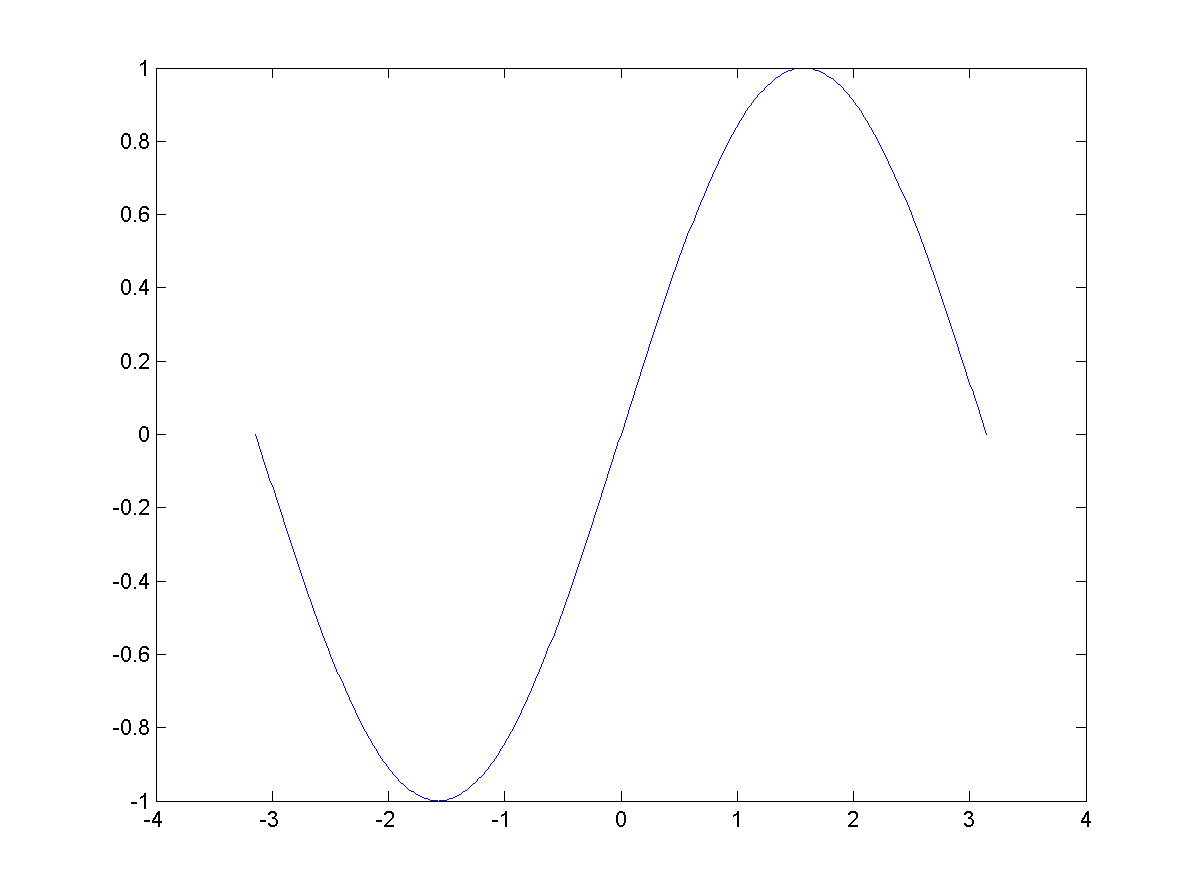
\includegraphics[scale=0.6]{src/ch4/img_4_1.png}
\captionof{figure}{Gráfica en 2D en coordenadas rectangulares}
\end{center}

\subsubsection{Graficar más de una función}

Si necesita incluir dos o más gráficas en una misma ventana puede utilizar el comando 
hold on para permitir que MATLAB simplemente agregue las gráficas sin borrar las ya 
existentes, por ejemplo:

\begin{verbatim}
	x=-pi:pi/180:pi;
	y1=sin(x);
	y2=cos(x);
	y3=cos(x+pi/3);
	hold on
	plot(x,y1);
	plot(x,y2);
	plot(x,y3);
\end{verbatim}

\begin{center}
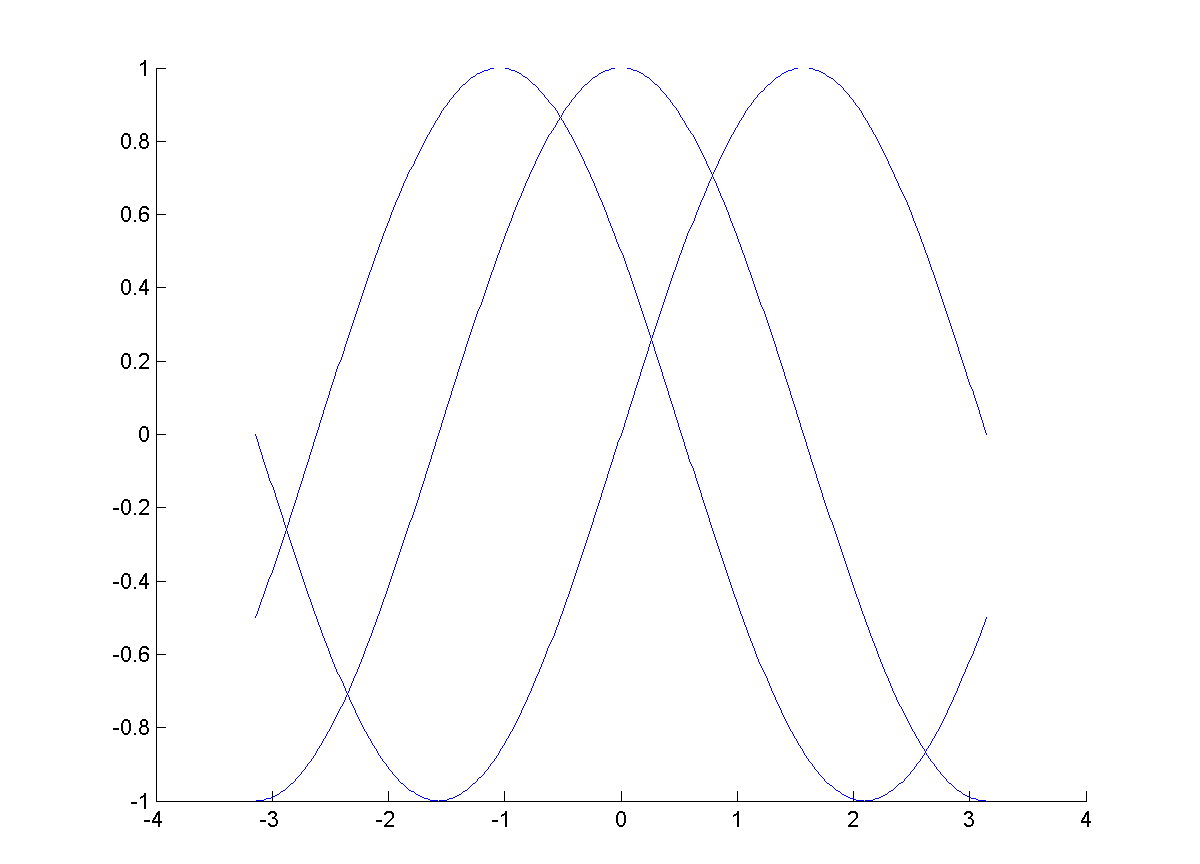
\includegraphics[scale=0.6]{src/ch4/img_4_2.png}
\captionof{figure}{Dos gráficas en una misma ventana}
\end{center}

Lo anterior funciona incluso para cuando se tienen intervalos diferentes. Si necesita 
graficar dos o más funciones en un mismo intervalo, es decir utilizando el mismo vector 
como variable independiente, puede utilizar la siguiente forma más compacta para agregar 
más de una función sin recurrir al comando descrito con anterioridad:

\begin{verbatim}
	x=-pi:pi/180:pi;
	y1=sin(x);
	y2=cos(x);
	y3=cos(x+pi/3);
	plot(x,[y1;y2;y3]);
\end{verbatim}

\begin{center}
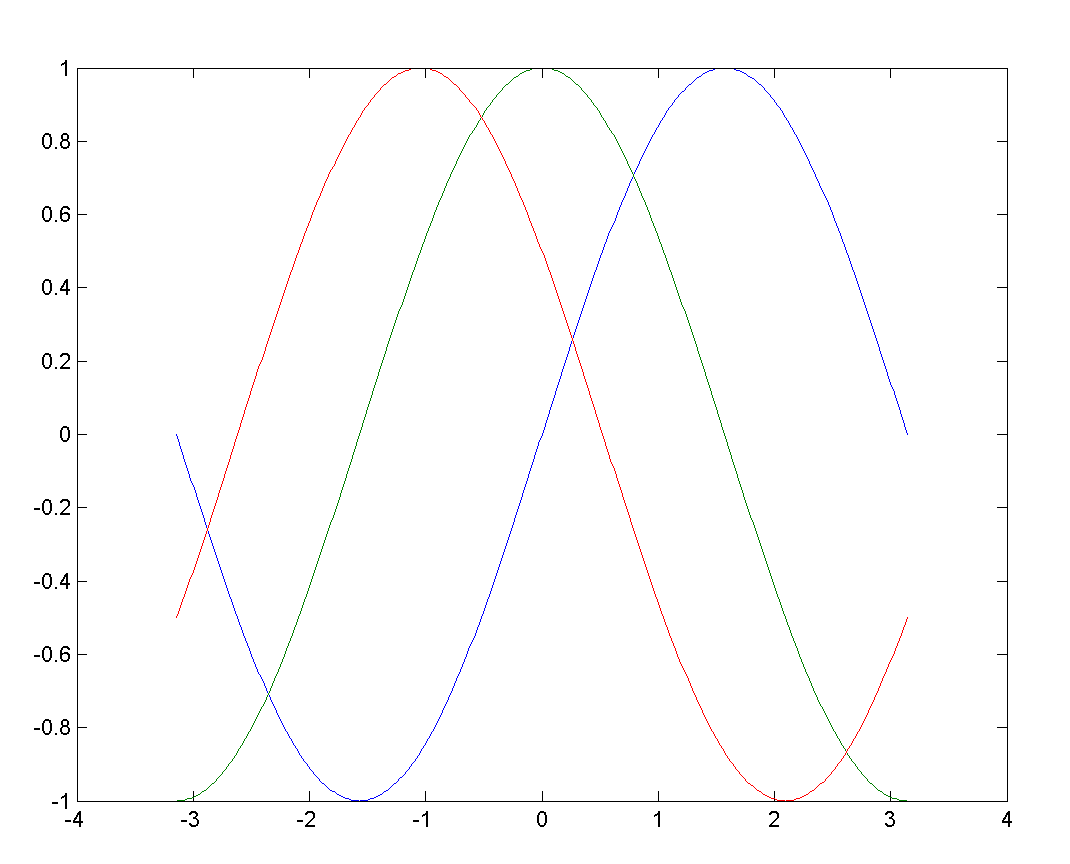
\includegraphics[scale=0.6]{src/ch4/img_4_3.png}
\captionof{figure}{Dos gráficas en una misma ventana}
\end{center}

En lugar de utilizar hold on puede configurar la propiedad NextPlot del axes de tal manera 
que las gráficas sean agregadas sin borrar los objetos que pertenecen al axes. Lo anterior 
se logra con la siguiente línea de código:

\begin{verbatim}
	set(gca,'NextPlot','add');
\end{verbatim}

Quizá lo anterior resulte un poco avanzado para comenzar, pero puede tomarse simplemente 
como una observación muy útil de que en MATLAB pueden implementarse diversas soluciones a 
un mismo problema o requerimiento.

\subsection{Configurar propiedades de las gráficas}

\subsubsection{Añadir etiquetas, leyendas y títulos}

En la sección anterior se han visto los pasos para mínimos para trazar una gráfica, pero 
ésta todavía puede resultar poco útil dado que no contiene información de ningún tipo 
acerca de los datos graficados. Es posible añadir etiquetas a los ejes con las funciones 
xlabel, ylabel y zlabel, además de poder añadir una identificación de una determinada 
curva mediante la función \texttt{legend} e incluso colocar un título en la parte superior con la 
función \texttt{title}:

\begin{verbatim}
	x=-pi:pi/180:pi;
	y=sin(x);
	plot(x,y);
	xlabel('Eje X');
	ylabel('Eje Y');
	title('Gráfica función seno');
	legend('f(x)=sin(x)');
\end{verbatim}

\begin{center}
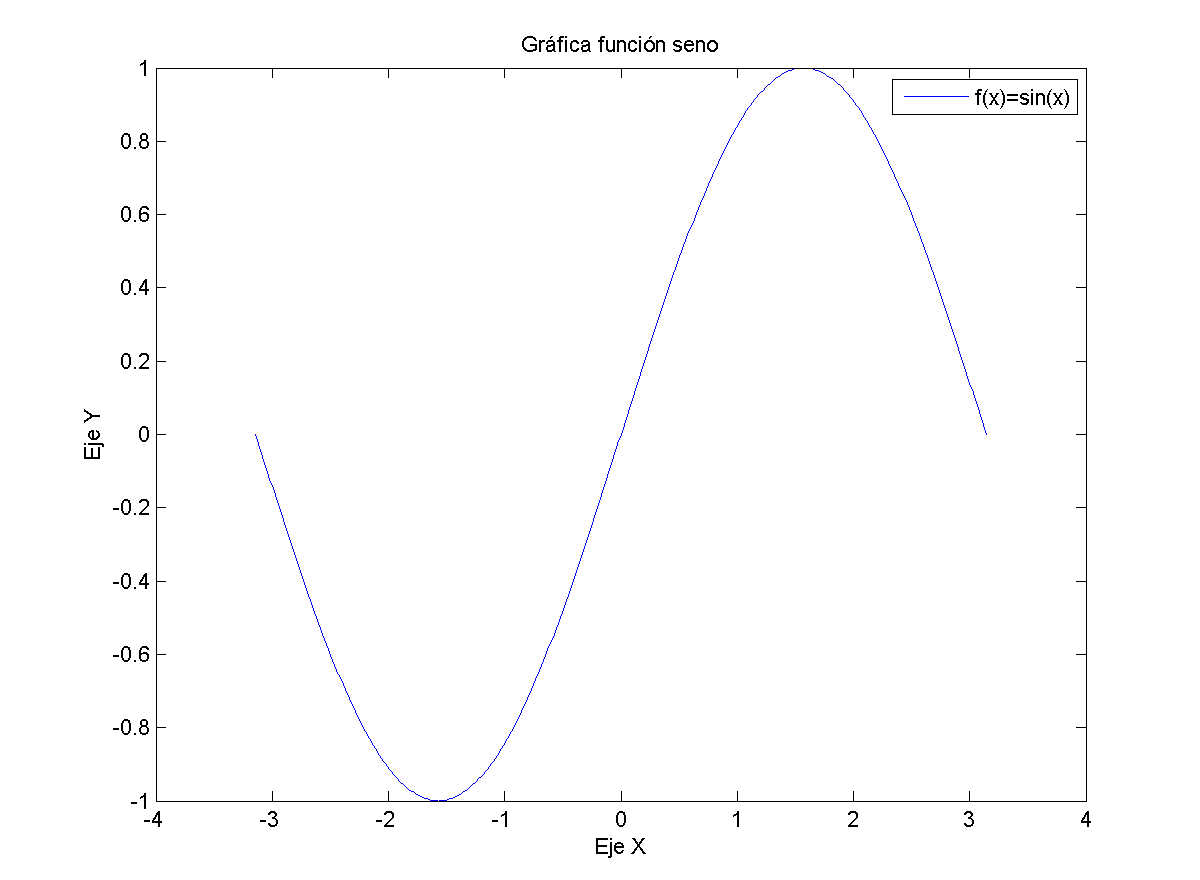
\includegraphics[scale=0.6]{src/ch4/img_4_4.png}
\captionof{figure}{Añadiendo etiquetas y título}
\end{center}

Las gráficas anteriores se han trazado utilizando el estilo por defecto que emplea MATLAB, 
es decir, una línea continua en color azul, pero  es posible modificar el color, grosor y 
el estilo de línea de las gráficas de modo que se ajuste a los requerimientos o a las 
exigencias visuales de cada individuo.

\subsubsection{Modificando el color de línea}

Para modificar el color de una gráfica basta con añadir como tercer argumento de la 
función plot uno de los modificadores de color que se indican en la siguiente tabla:

\begin{table}[h!]
\centering
{\rowcolors{1}{}{gray!20}
\begin{tabular}{p{4cm} p{4cm}}\hline
\rowcolor{LightBlue2} COLOR & MODIFICADOR \\
Rojo & \texttt{'r'} \\
Verde & \texttt{'g'} \\
Azul & \texttt{'b'} \\
Cyan & \texttt{'c'} \\
Magenta & \texttt{'m'} \\
Amarillo & \texttt{'y'} \\
Negro & \texttt{'k'} \\ 
Blanco & \texttt{'w'} \\
\end{tabular}
\caption{Modificadores de color}
\end{table}

La sintaxis de la función plot para una línea color verde sería:

\begin{verbatim}
	plot(x,y,'g');
\end{verbatim}

Además de los modificadores anteriores puede utilizarse un vector de tres elementos 
RGB para especificar el color, pero en este caso tiene que especificarse como argumento 
la propiedad que se modifica, es decir color, con lo cual la sintaxis bajo este método 
para trazar una línea color verde sería como sigue:

\begin{verbatim}
	plot(x,y,'color',[0 1 0]);
\end{verbatim}

\subsubsection{Configurar ejes (función axis)}

El comando / función axis permite hacer modificaciones a la apariencia y escala de los 
ejes en los cuales se trazan las gráficas. La sintaxis varía dependiendo de la 
característica a modificar.\\

\textit{Estableciendo los límites de una gráfica}\\

Para establecer los límites en los cuales se mostrará una gráfica puede introducir 
como argumento de la función axis un vector de 4 (gráficas en 2D) o 6 elementos 
(gráficas en 3D) con la sintaxis:

\begin{verbatim}
	axis([xmin xmax ymin ymax]); % Dos dimensiones
	axis([xmin xmax ymin ymax zmin zmax]); % Tres dimensiones
\end{verbatim}

Los elementos del vector deben ser de tipo double.\\

\textit{Ocultar o mostrar etiquetas, marcas, y ejes}\\

Si requiere ocultar los ejes, etiquetas, leyendas y demás marcas en las gráficas, de tal 
manera que sólo sea visible la línea trazada, utilice la función axis con el argumento 
\texttt{'off'}. Las siguientes líneas de código producen la imagen adjunta:

\begin{verbatim}
	x=linspace(-2*pi,2*pi,200);
	y=x.*cos(x);
	plot(x,y);
	axis off
\end{verbatim}

\begin{center}
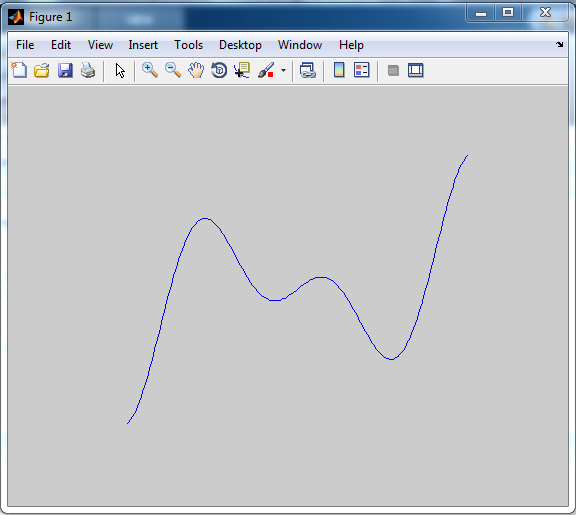
\includegraphics[scale=0.6]{src/ch4/img_4_5.png}
\captionof{figure}{Ocultando los ejes}
\end{center}

\textit{Escalado de ejes}\\

Además de permitir una configuración manual de los límites de ejes mediante la inserción 
de valores, es posible también establecer límites mediante modificadores que configuran 
los ejes y su apariencia de forma predeterminada. Los más comunes se enlistan y describen 
en la tabla siguiente.

\begin{table}[h!]
\centering
{\rowcolors{1}{}{gray!20}
\begin{tabular}{p{4cm} p{10cm}}\hline
\textbf{SINTAXIS} & \textbf{DESCRIPCIÓN} \\
\texttt{axis('equal')} & Ajusta el escalado de los ejes de tal modo que sean iguales en cada dirección. \\
\texttt{axis('square')} & Configura y ajusta la visualización de los ejes a un cuadrado o cubo (3D) \\
\texttt{axis('tight')} & Ajusta los ejes al rango de datos disponibles. \\
\end{tabular}
\caption{La función axis}
\end{table}

\subsubsection{Añadir anotaciones}

\subsection{Gráficas en coordenadas polares}

En el sistema de coordenadas polares cada punto del plano está definido por un ángulo y 
una distancia medidos respecto al eje polar y al polo, respectivamente. Generalmente para 
la notación de una ecuación polar se utilizan la letra griega $\theta$ para el ángulo 
y una r o $\rho$ para designar la distancia, siendo común la designación $r(\theta)$ para 
referir a una función en coordenadas polares.

Para graficar en coordenadas polares MATLAB dispone de la función polar cuya sintaxis es:

\begin{verbatim}
	polar(theta,rho);
\end{verbatim}

Ejemplo. Grafique la ecuación   (espiral)

\begin{verbatim}
	theta=0:pi/180:6*pi;
	r=theta;
	polar(theta,r);
\end{verbatim}

\begin{center}
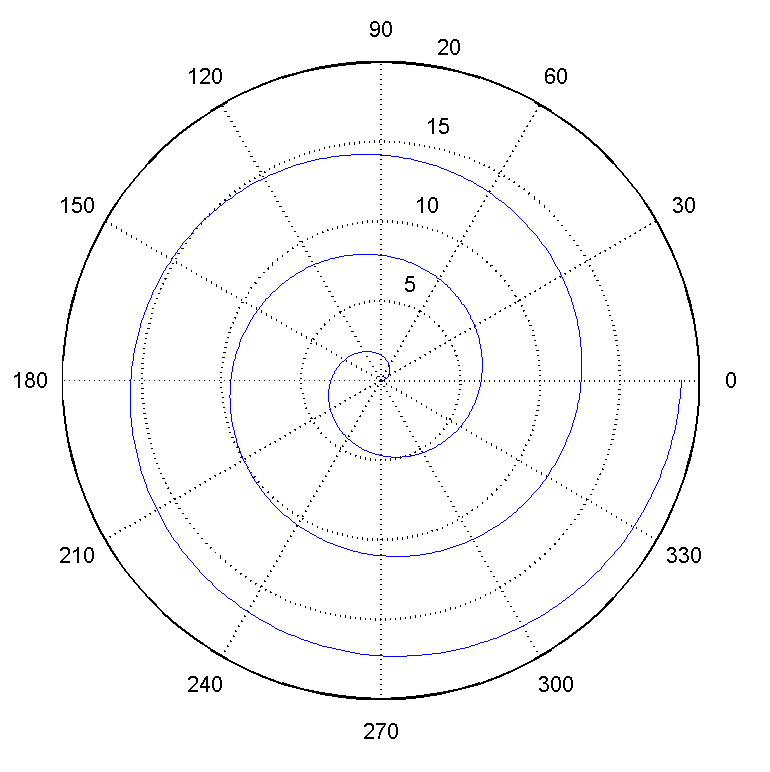
\includegraphics[scale=0.6]{src/ch4/img_4_6.png}
\captionof{figure}{Gráfica de una espiral en coordenadas polares}
\end{center}

Pese a que MATLAB cuenta con la función polar para facilitar el trazado de gráficas en 
coordenadas polares, es muy sencillo graficar estas utilizando la función plot con una 
conversión de coordenadas previa, por ejemplo, para la misma función anterior:

\begin{verbatim}
	theta=0:pi/180:6*pi;
	r=theta;
	x=r.*cos(theta); % Conversión de coordenadas 
	y=r.*sin(theta);
	plot(x,y);
\end{verbatim}

\section{Gráficas en tres dimensiones}

\subsection{Gráficas de superficies: una primera aproximación}

La representación gráfica de una función de dos variables $f(x,y)$ es una superficie 
trazada en un espacio tridimensional, resultante de la evaluación de la función en 
intervalos determinados para cada variable independiente.\\

A manera de ejemplo crearemos una matriz con los valores resultantes de la evaluación 
de la función en un punto específico; comenzaremos definiendo una función anónima de 
dos variables y enseguida utilizar ciclos for anidados para evaluar la función en 
cada punto. Véase el ejemplo mostrado a continuación:

\begin{verbatim}
	f=@(x,y) x.^2+y.^2;
	X=-5:0.2:5;
	Y=-5:0.2:5;
	for i=1:length(X)
	    for j=1:length(Y)
	        Z(i,j)=f(X(i),Y(j));
	    end
	end
	surf(Z);
\end{verbatim}

\begin{center}
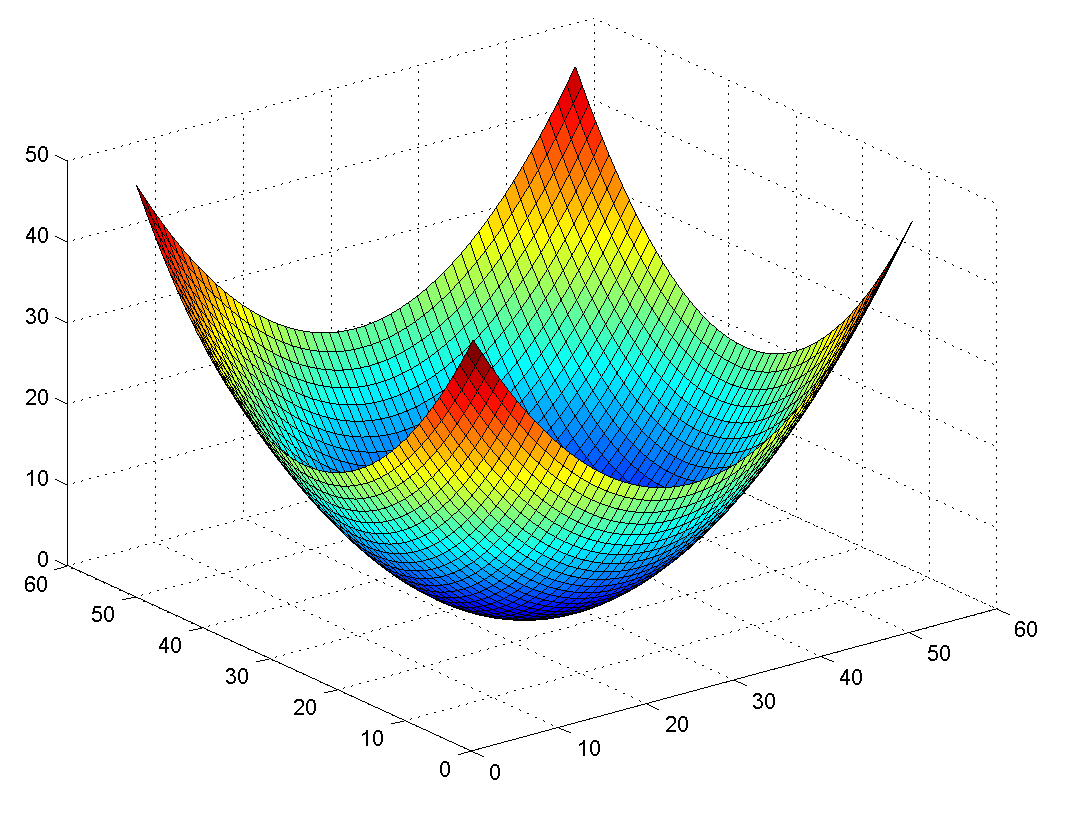
\includegraphics[scale=0.6]{src/ch4/img_4_7.png}
\end{center}

La función \texttt{surf} en el ejemplo anterior recibe como argumento de entrada una matriz bidimensional 
cuyos valores corresponden a cada punto evaluado. El código mostrado es funcional y muy entendible 
para un usuario que comienza en el mundo MATLAB, e incluso podría hacerse más "portable" o "reutilizable" 
si se definiese como una función, pero presenta ciertos inconvenientes: los ciclos for en MATLAB son 
generalmente conocidos por su lentitud, y más aún, en este caso se tienen dos ciclos for anidados. 
Debido a ello, MATLAB proporciona funciones que realizan la "tarea" de evaluar una función de dos 
variables en un rango definido mediante la implementación de rejillas bidimensionales (meshgrid), estas 
funciones se encuentran optimizadas mediante la técnica de vectorización y permiten una ejecución 
notablemente más veloz.

\subsection{Gráficas de superficies}

En el apartado anterior se ha visto como trazar superficies utilizando ciclos for anidados para crear 
la matriz que define los valores de la función de dos variables, pero ahora vamos a optimizar nuestro 
código utilizando la función \texttt{meshgrid} para definir el rango de valores a evaluar, la sintaxis 
de \texttt{meshgrid} es:

\begin{verbatim}
	>> [X,Y]=meshgrid(ix,iy);
\end{verbatim}

Donde X e Y son las matrices que definen el rango para las variables independiente y que se utilizarán 
para evaluar en una determinada función, ix e iy son vectores que definen el intervalo a evaluar de 
cada variable independiente. A continuación se muestra un ejemplo completo de cómo utilizar meshgrid 
en conjunto con surf para crear una gráfica de la función $f(x,y)=cos(x) sin(y)$:

\begin{verbatim}
	ix=0:0.2:10;
	iy=-5:0.2:5;
	[X,Y]=meshgrid(ix,iy);
	Z=cos(X).*sin(Y);
	surf(X,Y,Z);
\end{verbatim}

\begin{center}
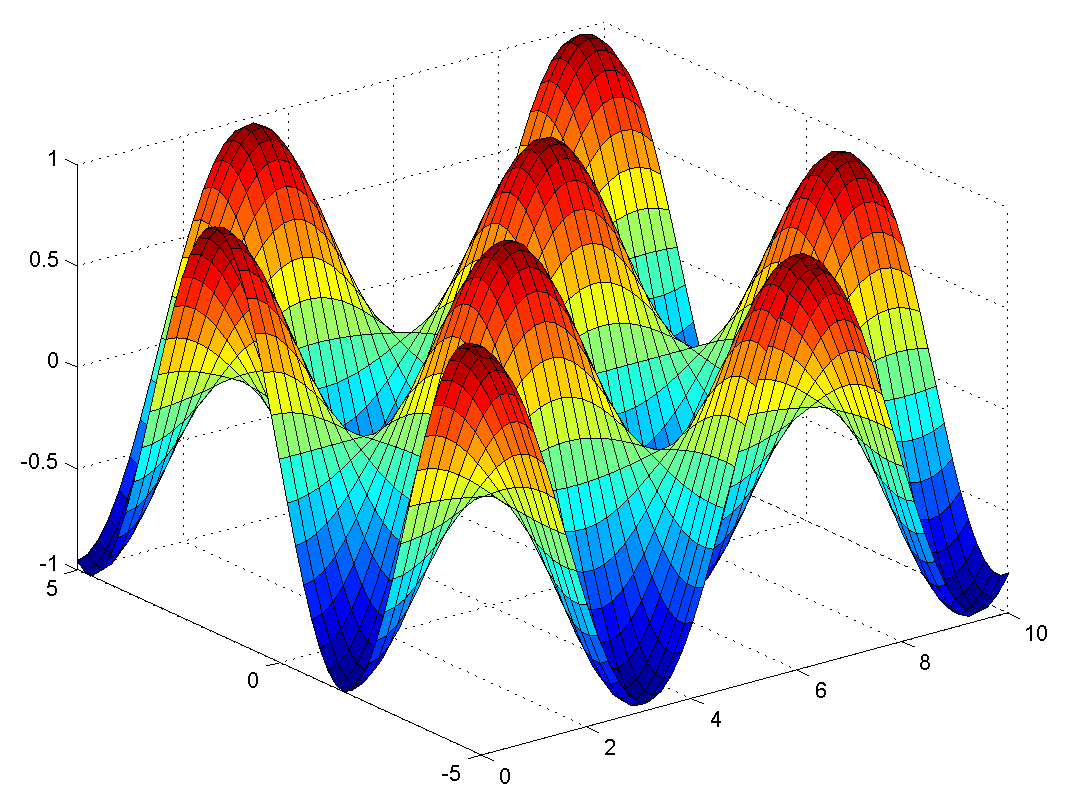
\includegraphics[scale=0.6]{src/ch4/img_4_8.png}
\end{center}

Note  que las operaciones de multiplicación o división deben estar vectorizadas, es decir, 
colocar un punto antes de cada operador correspondiente para indicar que se debe operar 
elemento a elemento. De lo contrario MATLAB devolverá un error o más grave aún: un resultado incorrecto.\\

Si ambos intervalos X e Y son iguales, puede proporcionar solo un argumento a la 
función meshgrid, es decir, es lo mismo tener esto:

\begin{verbatim}
	[X,Y]=meshgrid(1:10,1:10);
\end{verbatim}

que lo siguiente:

\begin{verbatim}
	[X,Y]=meshgrid(1:10);
\end{verbatim}

Claro que por cuestiones de comodidad sería preferible esta última, aunque quizá afecte 
un poco la legibilidad de un programa de mayores dimensiones, pero vamos, nada "catastrófico".

\subsection{Mapas de colores, sombreado e iluminación}

\subsubsection{Mapas de colores}

Un mapa de color es, en su definición más simplista, una matriz de m x 3 elementos 
cuyos valores se encuentran en el intervalo de 0 a 1, y donde cada fila representa 
un vector que especifica un color en el formato o modelo de color RGB. Pero, aquí 
la cuestión interesante es ¿para qué sirve un mapa de color?; así pues, un mapa de 
color no es más que un conjunto de colores que habrán de utilizarse para "pintar" 
una superficie de acuerdo a sus valores, pudo notar que en las superficies trazadas 
en los apartados anteriores se utiliza un color rojo para los valores más grandes y 
un color azul para los más pequeños, pasando por otras tonalidades para valores 
intermedios. Debe saber que esa "forma de colorear" la superficie está definida 
mediante un mapa de color por defecto, generalmente jet. Aparte de jet MATLAB 
cuenta con otros mapas de colores predefinidos que se muestran a continuación:

\begin{center}
\includegraphics[scale=1]{src/ch4/img_4_9.png}
\end{center}

Si teclea en MATLAB el nombre de cualquiera de los mapas de colores mostrados se devuelve 
una matriz de 64x3 elementos de tipo double, por ejemplo:

\begin{verbatim}
	>> map_color=hsv;
	>> whos map_color
	  Name            Size            Bytes  Class     Attributes

	  map_color      64x3              1536  double          
\end{verbatim}

Pero todo esto no tiene efecto sobre alguna superficie dibujada, para cambiar o configurar 
el mapa de color actual puede utilizar la función \texttt{colormap}, pasando un mapa de color como 
argumento, por ejemplo:

\begin{verbatim}
	[X,Y]=meshgrid(0:0.2:3*pi);
	Z=cos(X).*sin(Y);
	surf(X,Y,Z);
	colormap(hot);
\end{verbatim}

\begin{center}
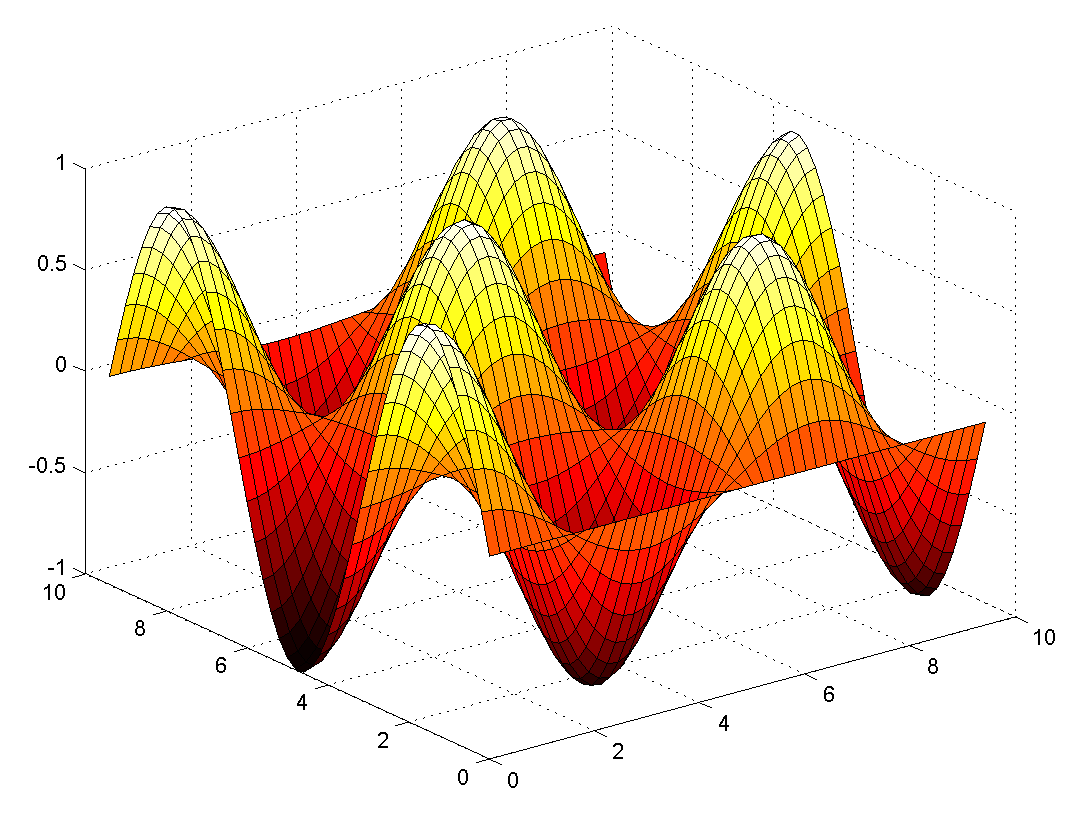
\includegraphics[scale=0.6]{src/ch4/img_4_10.png}
\end{center}

Interesante, sobre todo para quienes deseen darle a sus gráficos una mayor calidad 
estética o acorde a los datos que esté representando.\\

Si por alguna razón ninguno de los mapas de colores predefinidos le "convence", puede 
definir su propio mapa de color sin muchas complicaciones, para ello debe crear una 
matriz de m x 3 elementos donde cada fila contenga información acerca de un color en 
formato RGB, tomando en cuenta que el color ubicado en la primera fila será asignado 
al valor más pequeño y la última fila al mayor. Revise el siguiente ejemplo en el 
cual se define un mapa de color mediante cierta secuencia:

\begin{verbatim}
	Z=membrane;
	surf(Z);
	v=(1:10)'/10;
	cmap=[v flipud(v) flipud(v)];
	colormap(cmap);
\end{verbatim}

\begin{center}
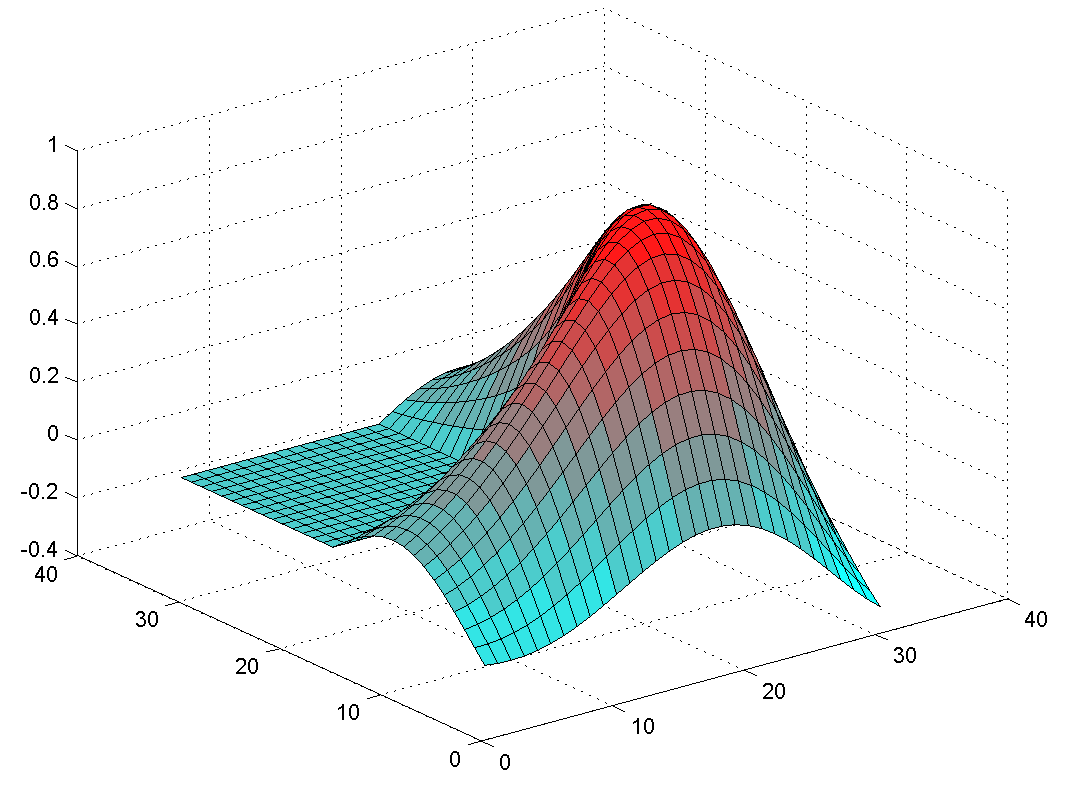
\includegraphics[scale=0.6]{src/ch4/img_4_11.png}
\end{center}

El resultado es una interesante variación de tonalidades ¿azul? a rojo. Por supuesto 
que  usted tiene todas las libertades para experimentar con diversas secuencias de 
colores y "adoptar" la que mejor le resulte.

\subsubsection{Sombreado}

Para efectos de esta sección, con sombreado se refiere a la forma en que MATLAB 
\textit{pinta} o \textit{rellena} los diversos componentes o parches (patch) que 
conforman una superficie.\\

En MATLAB existen tres tipos de sombreado que pueden controlarse mediante la función 
\texttt{shading}, los cuales son:

\begin{itemize}
\item faceted
\item flat
\item interp
\end{itemize}

El tipo \texttt{faceted} es el sombreado por defecto, y se caracteriza por pintar cada 
parche de la superficie utilizando un color sólido de relleno y un borde en color negro.\\

El tipo \texttt{flat} funciona de manera similar al anterior, con la diferencia que el borde 
adquiere el mismo color que el interior del parche.\\

Y el tipo \texttt{interp} se vale de una interpolación de la matriz que define el mapa de 
color actual para pintar de forma cuasi-continua y con variaciones menos "bruscas" a 
cada parche, de hecho con este tipo de sombreado es imposible distinguir cada pieza 
que compone la superficie.\\

La función \texttt{shading} sólo necesita como argumento el tipo de sombreado, por ejemplo:

\begin{verbatim}
	>> shading('flat')
\end{verbatim}

Incluso acepta la notación de comandos, es decir, la siguiente forma también es válida:

\begin{verbatim}
	>> shading flat
\end{verbatim}

\subsubsection{Iluminación}

\section{Animaciones}

\subsection{Mi primera animación, una introducción}

Quizá parezca un poco lógico que para realizar una animación debe hacerse uso de bucles 
(for o while), dado que estos permiten variaciones durante el tiempo que se ejecutan. 
Tómese como ejemplo el siguiente código:

\begin{verbatim}
	x=0:0.01:10;
	for i=1:10
	    plot(x,sin(x+i));
	end
\end{verbatim}

Si ejecuta el código anterior comprobará que únicamente le será visible la última 
gráfica que corresponde al valor de i=10, es decir de la función   ; las demás gráficas 
también se muestran pero durante un lapso de tiempo demasiado breve como para percibirlo. 
Para ralentizar la ejecución del bucle for puede utilizarse la función pause que permite 
detener la ejecución de un programa durante un periodo de tiempo especificado en segundos; 
modificando el código anterior podemos “mejorar” nuestra animación.

\begin{verbatim}
	x=0:0.01:10;
	for i=1:10
	    plot(x,sin(x+i));
	    pause(0.1);
	end
\end{verbatim}

Ahora es posible visualizar el cambio efectuado en cada ejecución del ciclo for, siendo en 
este caso el desplazamiento de la función seno; en cada  ciclo MATLAB detiene durante 0.1 
segundos la ejecución, lo que permite al usuario visualizar cada una de las gráficas como 
un continuo animado.\\

Una vez conocido lo anterior, podemos añadir variaciones no solamente en la forma, sino 
también en el color de la gráfica utilizando vectores formados por valores aleatorios en 
cada secuencia, por ejemplo una modificación de ese tipo sería:

\begin{verbatim}
	x=0:0.01:10;
	for i=1:10
	    plot(x,sin(x+i),'linewidth',2,'color',rand(1,3));
	    set(gca,'color',rand(1,3));
	    pause(0.1);
	end
\end{verbatim}

Verifique los resultados de la animación. Claro que las modificaciones que pueden hacerse 
dependen de la imaginación, creatividad o de la necesidad de cada usuario. En la siguiente 
imagen se muestra la secuencia correspondiente a la animación.

\begin{center}
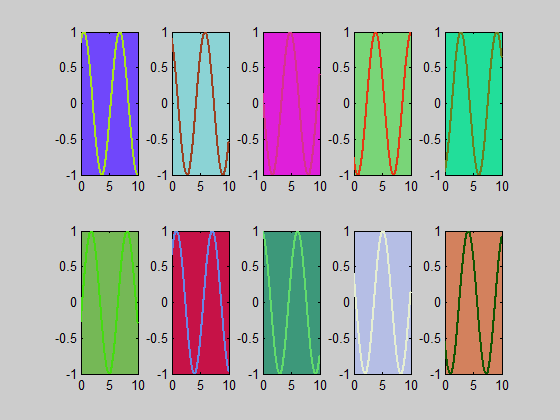
\includegraphics[scale=0.6]{src/ch4/img_4_12.png}
\end{center}
\chapter{Exportar e importar variables y datos}

\section{Guardar y cargar variables del workspace: save y load}

Durante una sesión ordinaria utilizando MATLAB las variables creadas se almacenan en el 
workspace y están disponibles para usarse, siempre y cuando no se haya utilizado algún 
comando para borrar las variables, sin embargo cuando se cierra la sesión de MATLAB las 
variables del workspace son borradas y no es posible utilizarlas posteriormente. Para 
poder “conservar” una variable creada y utilizarla en cálculos futuros, es posible 
guardar estas en archivos MAT nativos del lenguaje MATLAB; lo anterior se logra utilizando 
la función save, cuya sintaxis es:

\begin{verbatim}
	save('nomb_arch.mat','nvar');
\end{verbatim}

Siendo \texttt{nomb\_arch} el nombre del archivo en el cual se guardarán las variables, 
que incluso puede ser una combinación de una dirección absoluta o relativa y el nombre 
del archivo; nvar es el nombre de la variable o variables a ser guardadas. Si desea 
guardar todas las variables actuales puede omitir el resto de argumentos y solo 
utilizar el nombre del archivo. Las siguientes líneas ejemplifican cómo hacer uso 
de la función save:

\begin{verbatim}
	>> k=1.37;
	>> A=[1 2 -1;0 1 0;-2 0 0];
	>> C={'A','B','C'};
	>> save('arch1.mat'); % Guarda todas las variables
	>> save('arch2.mat','A'); % Guarda sólo la variable A
\end{verbatim}

El contenido de los archivos MAT puede cargarse y guardar en el workspace mediante 
la función \texttt{load}, con la sintaxis:

\begin{verbatim}
	load('narch.mat','vars');
\end{verbatim}

Donde narch es el nombre del archivo y vars la(s) variable(s) a cargar en el workspace. 
Si únicamente se indica como argumento el nombre del archivo, entonces se cargan todas 
las variables contenidas en el archivo. Para ejemplificar el uso de load utilizaremos 
el archivo “arch1.mat” creado anteriormente:

\begin{verbatim}
	>> load('arch1.mat');
	>> whos % Verificamos las variables cargadas en el workspace
	  Name      Size            Bytes  Class     Attributes
	  A         3x3                72  double              
	  C         1x3               342  cell                
	  k         1x1                 8  double       
\end{verbatim}

Puede asignarse la función load a una variable, con lo cual todo el contenido del 
archivo MAT se guardara en una estructura con cada una de las variables como campos. 
Para el mismo ejemplo anterior se tiene:

\begin{verbatim}
	>> S=load('arch1.mat');
	>> S
	S = 
	    k: 1.3700
	    A: [3x3 double]
	    C: {'A'  'B'  'C'}
	>> whos 
	  Name      Size            Bytes  Class     Attributes
	  S         1x1               950  struct       
\end{verbatim}


\section{Carpetas y archivos, operaciones básicas.}

\subsection{Cambiar el directorio o carpeta actual}

La función cd cambia la carpeta actual (Current Folder), utilizando como argumento 
una cadena de caracteres con la dirección absoluta o relativa del nuevo directorio 
de trabajo. La sintaxis es:

\begin{verbatim}
	cd('Nueva Carpeta');
\end{verbatim}

Un ejemplo se muestra enseguida:

\begin{verbatim}
	cd('C:\Users\User\Documents\MATLAB');
\end{verbatim}

Si solo se pone la instrucción \texttt{cd} sin argumentos, entonces MATLAB devuelve un 
string con la carpeta actual.

\begin{quote}
\textbf{Direcciones absolutas y relativas}.\\
Una dirección absoluta es aquella representada mediante toda la ruta que la describe, 
incluyendo al directorio raíz. En Windows las direcciones absolutas suelen ser de la forma 
\texttt{C:/Users/User/…}, donde User es el nombre del usuario registrado en el equipo.
Las direcciones relativas se expresan con respecto a una determinada carpeta, por ejemplo, 
si estamos ubicados dentro de una carpeta Documents cuya dirección absoluta es 
\texttt{C:/Users/User/Documents} y dentro de ella tenemos una carpeta llamada MATLAB, la forma 
relativa de referirnos a esta carpeta sería simplemente con la cadena \texttt{'\MATLAB'}.
\end{quote}

\subsection{Crear y eliminar carpetas}

A estas alturas, crear y manipular carpetas resulta una tarea trivial cuando se ejecuta 
en el ambiente de cualquier sistema operativo que maneje, incluso en el Current Folder 
de MATLAB puede crear, modificar y eliminar carpetas tal como lo hace normalmente. Pese 
a lo anterior, en diversas situaciones puede ser necesario crear carpetas mediante la 
ejecución de código a través de comandos y/o funciones destinadas para tal fin. En MATLAB 
se dispone de la función mkdir que permite crear carpetas utilizando el nombre de la 
misma como argumento, por ejemplo:

\begin{verbatim}
	>> mkdir('Mis Cursos');
\end{verbatim}

La instrucción anterior crea una carpeta llamada Mis Cursos en el directorio actual de 
trabajo. Es posible también pasar como argumento la dirección absoluta o relativa de 
la carpeta a crear:

\begin{verbatim}
	>> mkdir('Mis Cursos/MATLAB');
\end{verbatim}

En la línea anterior se crea dentro de la carpeta Mis Cursos una cuyo nombre es MATLAB.

Habitualmente en la programación se hace necesario considerar la mayoría de las 
situaciones posibles para dar una mayor robustez al código, y con ello hacerlo más 
autónomo y eficiente. Imagine que necesite crear carpeta a la cual le asignará un 
nombre determinado, entonces, hay una posibilidad, aun siendo mínima, que ya exista 
una carpeta con ese mismo nombre. MATLAB no remplazará la carpeta existente por la nueva, 
pero le mostrará un mensaje de error o advertencia y posiblemente detenga la ejecución 
del código. Para evitar lo anterior puede comprobar antes si existe un directorio con 
ese nombre y mediante una sentencia de control especificar las acciones a ejecutar en 
cada caso. Véase el ejemplo siguiente en donde se realiza la comprobación mediante 
la función isdir:

\begin{verbatim}
	if ~isdir('Cursos')
	    mkdir('Cursos');
	else
	    mkdir(['Cursos','2']);
	end
\end{verbatim}

Para eliminar una carpeta MATLAB proporciona la función rmdir cuyo argumento es la 
carpeta a eliminar, o bien la dirección absoluta o relativa de la misma. Por ejemplo, 
si quiere eliminar una carpeta llamada Cursos, ubicada en el directorio actual:

\begin{verbatim}
	>> rmdir('Mis Cursos');
\end{verbatim}

Lo anterior funciona para carpetas que no contengan subcarpetas, de lo contrario 
MATLAB le devolverá un mensaje de error como el siguiente:

\begin{verbatim}
	>> rmdir('Mis Cursos')
	Error using rmdir
	No directories were removed.
\end{verbatim}

Para borrar una carpeta que contenga subcarpetas debe incluir un segundo argumento, 
siendo este una “s” entre comillas simples, como se muestra:

\begin{verbatim}
	>> rmdir('Mis Cursos','s');
\end{verbatim}

\subsection{Crear y eliminar carpetas}

Conocer los archivos y directorios dentro de una carpeta suele ser una necesidad 
básica para cualquier programador, sobre todo para el almacenamiento y organización 
de archivos de trabajo. MATLAB cuenta con funciones que facilitan la tarea de consultar 
el contenido de una carpeta, entre las más comunes están dir, ls y what, a continuación 
veremos la utilidad de cada una.

\subsubsection{La función dir}

La función dir, sin argumentos de salida pedidos de forma explícita y sin argumentos 
de entrada, devuelve en pantalla una lista de archivos y directorios contenidos en 
el \textbf{Current Folder}. Véase el ejemplo:

\begin{verbatim}
	>> dir
	.               grlev.png       matricesEx.m    
	..              idmat.m         ordseleccion.m  
	datos.txt       img.png         unos.m     
\end{verbatim}

No obstante, si asignamos la función dir a una variable cualesquiera entonces se 
guardará una estructura que contiene información acerca del nombre, tamaño, fecha 
de modificación, entre otras características de los archivos contenidos en el 
directorio actual.

\begin{verbatim}
	>> S=dir
	S = 
	9x1 struct array with fields:
	    name
	    date
	    bytes
	    isdir
	    datenum
\end{verbatim}

Para acceder a la información de cada archivo puede hacerlo mediante el índice 
correspondiente, por ejemplo:

\begin{verbatim}
	>> S(3)
	ans = 
	       name: 'datos.txt'
	       date: '01-oct-2014 15:13:46'
	      bytes: 74
	      isdir: 0
	    datenum: 7.3587e+05
\end{verbatim}

Desde luego que esta forma de utilizar la función dir es mucho más útil que aquella 
que simplemente muestra en pantalla la información.

Es posible además especificar como argumento la dirección de la cual se requiere 
información (una distinta al Current Folder) e inclusive utilizar comodines para 
visualizar solo archivos con una determinada extensión, por ejemplo:

\begin{verbatim}
   	>> dir('C:/Users/User/Documents/MATLAB/*.png')
	ayuda.png  img.png 
\end{verbatim}   

La instrucción anterior busca en la carpeta MATLAB todos los archivos con 
extensión PNG (imágenes), sin importar el nombre de estos, e ignora cualquier 
otro tipo de archivo o directorio ubicado en esta misma carpeta. Ahora, 
revise el siguiente ejemplo:

\begin{verbatim}
	>> dir('C:/Users/User/Documents/MATLAB/m*')
	MATLAB TYP           Mecanismos           My File Exchange     
	MATLAB_Function.m    Mis Apuntes          matrizBinaria.m      
	Matemáticas Básicas  Moler Books          miHist.m       
\end{verbatim}

Como puede observar, MATLAB devuelve todos aquellos archivos y carpetas cuya 
primera letra sea \textbf{m}, sin importar ninguna otra característica.

\subsection{Mover, copiar y eliminar archivos}

Mover, copiar y eliminar archivos son tareas muy comunes para cualquier usuario  
de un ordenador y que pueden ejecutarse con mucha facilidad de forma manual. No 
obstante, utilizar la programación para estas tareas puede resultar de mucha ayuda, 
sobre todo cuando se necesita trabajar con grandes volúmenes de datos y/o archivos, 
ya que permite automatizar los procedimientos y ejecutarlos en un tiempo impensable 
para un individuo. Claro que se podría justificar que existen formas para seleccionar 
todos los archivos de un directorio y colocarlos en otro de forma muy sencilla  aun 
cuando fuesen millares de archivos, pero ¿qué pasa si solo necesitamos trabajar con 
archivos cuyo nombre cumpla una determinada característica o patrón? ¿O con archivos 
de un tamaño específico? ¿O con una fecha de modificación reciente?, incluso con 
combinaciones de las anteriores posibilidades, de esa manera no es tan trivial 
seleccionar de forma manual archivos que cumplan tales condiciones, pero utilizando 
la programación puede solucionar de forma efectiva dichas situaciones.

MATLAB proporciona funciones que sirven para realizar las tareas mencionadas en el 
párrafo anterior. Con movefile y copyfile puede mover y copiar archivos de un directorio 
a otro, la sintaxis es muy similar, necesitando solamente el directorio origen y destino 
como argumentos de entrada. Usaremos movefile para ejemplificar, pero desde luego que esto 
será aplicable para copyfile con tan solo cambiar el nombre de la función.

\section{Exportar e importar datos de un fichero de texto}

Existen múltiples formatos para ficheros que almacenan datos o texto plano, siendo los 
más comunes el *.txt y el *.dat. Estos tipos de ficheros son muy utilizados en casi 
cualquier ámbito para guardar datos de cualquier tipo, con la ventaja de ser \textit{leíbles}
para una persona y, por supuesto, para la computadora. Por tanto, con frecuencia se hace 
necesario el hecho de importar y/o exportar información de un archivo de este tipo, además 
es muy común utilizar MATLAB como un entorno de visualización de datos generados a través 
de la adquisición mediante tarjetas o bien mediante otro software.

\subsection{Exportar datos con dlmwrite}

La función dlmwrite exporta el contenido de una matriz a un archivo de texto usando 
un delimitador o separador entre los elementos. La sintaxis más común es:

\begin{verbatim}
	>> dlmwrite(n_arch, M, 'delimitador');
\end{verbatim}

Donde \texttt{n\_arch} es el nombre del archivo en el cual se guardará la matriz M, utilizando 
como separador el carácter especificado en \texttt{'delimitador'}.
\chapter{Matemáticas con MATLAB}

\section{Manipulación algebraica}

\subsection{Definir variables simbólicas}

Para la manipulación de expresiones algebraicas MATLAB dispone de un toolbox especial, 
el Symbolic Math Toolbox, que  tiene la capacidad de trabajar con expresiones de manera 
simbólica. Para comenzar se debe conocer cómo definir una variable de tipo simbólico, 
esto puede hacerlo de la siguiente forma:

\begin{verbatim}
	>> x=sym('x')
	x =
	x
\end{verbatim}

Puede introducir el comando whos para verificar el tipo de variable creada:

\begin{verbatim}
	>> whos
	  Name      Size            Bytes  Class    Attributes
	  x         1x1               112  sym         
\end{verbatim}

Normalmente, si introduce una literal que no ha sido asignada a un valor numérico o que no 
se ha declarado como simbólica MATLAB devuelve un mensaje de error similar a esto:

\begin{verbatim}
	>> x
	Undefined function or variable 'x'.
\end{verbatim}

Una vez se ha definido una variable como simbólica puede utilizarla en conjunto con valores 
numéricos para formar expresiones algebraicas, por ejemplo:

\begin{verbatim}
	>> x=sym('x');
	>> x+2*cos(x)
	ans =
	x + 2*cos(x)
	>> x^3-3*x^2-x+2
	ans = 
	x^3 - 3*x^2 - x + 2
\end{verbatim}

Pueden definirse dos o más variables simbólicas en una misma línea de código utilizando el 
comando syms de la siguiente manera:

\begin{verbatim}
	>> syms x y z
\end{verbatim}

Para simplificar una expresión algebraica MATLAB proporciona la función simplify, cuyo 
argumento de entrada es la expresión a simplificar, por ejemplo:

\begin{verbatim}
	>> simplify(sin(x)^2+cos(x)^2)
	ans =
	1
\end{verbatim}

Debe tomar en cuenta que el resultado que la función simplify devuelve es de  tipo simbólico.

\subsection{Factorizar y expandir  expresiones algebraicas}

Las funciones factor y expand del \textbf{Symbolic Math Toolbox} permiten factorizar y 
expandir toda clase de expresiones algebraicas. Por ejemplo, si se tiene la expresión 
algebraica $ x^2+2x+1 $ y se requiere factorizarla. En MATLAB bastaría con utilizar 
la función factor como sigue:

\begin{verbatim}
	>> factor(x^2+2*x+1)
	ans =
	(x + 1)^2
\end{verbatim}

Utilizando la función expand en la expresión devuelta puede regresarse a la forma inicial:

\begin{verbatim}
	>> expand((x+1)^2)
	ans =
	x^2 + 2*x + 1
\end{verbatim}

\section{Resolver ecuaciones e inecuaciones}

Una ecuación es una igualdad matemática entre dos expresiones algebraicas en las que 
aparecen valores conocidos y una variable desconocida (incógnita), relacionados mediante 
operaciones matemáticas básicas, ejemplos de ecuaciones se muestran a continuación:

$$3x^2+2x-2=0$$

$$x+\frac{3}{7}=2$$

$$\cos(x)+sin(\frac{\pi}{2})=0$$

Las ecuaciones algebraicas sirven para modelar situaciones poco complejas pero que 
requieren el uso de la herramienta matemática para obtener una solución satisfactoria. 
Existen diversos métodos para resolver ecuaciones, los cuales se aplican dependiendo 
del tipo de ecuación, incluso hay fórmulas establecidas para algunos tipos de ecuaciones 
que minimizan el esfuerzo de cálculo.\\

MATLAB dispone de la función solve perteneciente al Symbolic Math Toolbox, la cual permite 
resolver ecuaciones, inecuaciones y sistemas de ecuaciones; la sintaxis general de 
la función solve es:
	
\begin{verbatim}
	solve(ec, var);
\end{verbatim}

Donde ec es una ecuación algebraica definida usando variables simbólicas y var es la 
incógnita respecto a la cual se resuelve la ecuación dada.\\

A manera de ejemplo se resolverá la siguiente ecuación lineal $ x+3=2 $:

\begin{verbatim}
	>> x=sym('x');
	>> solve(x+3==2,x)
	ans =
	-1
\end{verbatim}

Es importante hacer mención que para especificar una igualdad se utilizan dos signos, 
dado que un sólo signo hace referencia a una asignación.\\

Si no se especifica el segundo miembro de la igualdad, MATLAB asumirá que la expresión 
estará igualada a cero, es decir, para resolver la ecuación:

$$ x^2-2x-1=0 $$

Puede hacerlo de las diversas formas que enseguida se muestran:

\begin{verbatim}
	>> solve(x^2-2*x-1==0,x)
	ans =
	 2^(1/2) + 1
	 1 - 2^(1/2)
	>> solve(x^2-2*x-1,x)
	ans =
	 2^(1/2) + 1
	 1 - 2^(1/2)
	>> solve(x^2-2*x-1)
	ans =
	 2^(1/2) + 1
	 1 - 2^(1/2)
\end{verbatim}

Para resolver desigualdades o inecuaciones la sintaxis es prácticamente la misma, claro, 
sólo hay que utilizar los operadores relacionales mayor que o menor que en lugar del signo 
de igualdad. Por ejemplo, resolviendo la siguiente desigualdad $x+2>10$:

\begin{verbatim}
	>> solve(x+2>10,x)
	ans =
	Dom::Interval(8, Inf)
\end{verbatim}

MATLAB devuelve el intervalo solución para la inecuación, en este caso $(8,\infty)$. Para el caso 
de un intervalo cerrado MATLAB devuelve entre corchetes el valor del límite correspondiente, 
por ejemplo:

\begin{verbatim}
	>> solve(x+2>=10,x)
	ans =
	Dom::Interval([8], Inf)
\end{verbatim}

Un sistema de ecuaciones se compone de dos o más ecuaciones y un número equivalente de 
valores desconocidos, es posible resolver sistemas de ecuaciones utilizando también la 
función solve con la sintaxis siguiente:

\begin{verbatim}
	solve(ec1,ec2,ec3,…)
\end{verbatim}

Un ejemplo, resolver el siguiente sistema de ecuaciones:

$$ x+y=4 $$
$$ x-y=3 $$

\begin{verbatim}
	>> syms x y
	>> sol=solve(x+y==4,x-y==3)
	sol = 
	    x: [1x1 sym]
	    y: [1x1 sym]
\end{verbatim}

Para visualizar los resultados puede acceder a los campos de cada variable como se muestra enseguida:

\begin{verbatim}
	>> sol.x 
	ans =
	7/2
	>> sol.y
	ans =
	1/2
\end{verbatim}

\section{Números complejos}

Los números complejos \index{Números complejos} son una extensión de los números reales, se representan como la 
suma de un número real y un número imaginario, siendo este último un múltiplo real de la 
unidad imaginaria, cuya representación suele hacerse utilizando las letras i o j. MATLAB, 
por defecto considera a las letras j e i como unidades imaginarias, siempre y cuando no hayan 
sido asignadas a un valor específico. Por ejemplo, vea que sucede cuando teclea la letra 
i o j en la ventana de comandos:

\begin{verbatim}
	>> i
	ans =
	        0 + 1.0000i
	>> j
	ans =
	        0 + 1.0000i
	>> whos
	  Name      Size            Bytes  Class     Attributes
	  ans       1x1                16  double    complex   
\end{verbatim}

Para crear un número complejo en su forma rectangular puede hacer uso de cualquiera de 
las siguientes formas que producen un resultado equivalente:

\begin{verbatim}
	>> Z=3+2i
	Z =
	   3.0000 + 2.0000i
	>> Z=complex(3,2)
	Z =
	   3.0000 + 2.0000i
\end{verbatim}

Es posible obtener la parte real e imaginaria de un número complejo utilizando las 
funciones real e imag respectivamente, véase el ejemplo a continuación:

\begin{verbatim}
	>> z=4+5i;
	>> real(z)
	ans =
	     4
	>> imag(z)
	ans =
	     5
\end{verbatim}

\section{Cálculo diferencial e integral}

\subsection{Límites}

Para calcular límites en MATLAB se tiene la función limit \index{limit} cuya sintaxis es:

\begin{verbatim}
limit(f,x,a)
\end{verbatim}

Donde f es la función a calcular el límite, x la variable independiente en cuestión, 
y a el valor al cual tiende la variable independiente, es decir, expresado en 
notación más amable sería:

$$ \lim_{x \to a} f(x) $$

Compute los siguientes ejemplos y verifique los resultados:

\begin{verbatim}
	>> limit(sin(x)/x,x,0)
	ans =
	1
	>> limit((x-2)/(x+3),x,-3)
	ans =
	NaN
	>> limit(exp(-x)+2,x,inf)
	ans =
	2
\end{verbatim}

La función limit acepta argumentos adicionales para calcular límites laterales por la 
izquierda y derecha, siendo estos las cadenas \texttt{'left'} y \texttt{'right'}. Revise los 
siguientes ejemplos:

\begin{verbatim}
	>> limit(1/(x-3),x,3,'left')
	ans =
	-Inf
	>> limit(1/(x-3),x,3,'right')
	ans =
	Inf
\end{verbatim}

\subsection{Derivadas}

Es pertinente mencionar que MATLAB dispone de dos funciones llamadas diff, una 
acepta un vector numérico como argumento de entrada, y la otra una expresión simbólica, 
de esta última nos ocuparemos en esta sección. Para solicitar ayuda con la sintaxis de 
esta función puede utilizar:

\begin{verbatim}
	>> help sym/diff
	 diff   Differentiate.
	    diff(S) differentiates a symbolic expression S with respect to its
	    free variable as determined by SYMVAR.
	    diff(S,'v') or diff(S,sym('v')) differentiates S with respect to v.
	    diff(S,n), for a positive integer n, differentiates S n times.
	    diff(S,'v',n) and diff(S,n,'v') are also acceptable.
	 
	    Examples;
	       syms x t
	       diff(sin(x^2)) is 2*x*cos(x^2)
	       diff(t^6,6) is 720.
	 
	    See also sym/int, sym/jacobian, sym/symvar.
\end{verbatim}

La función diff \inde{diff} del \textbf{Symbolic Math Toolbox} tiene una sintaxis general como sigue:

\begin{verbatim}
	>> df = diff(f,var)
\end{verbatim}

Donde f es la función a derivar, var la variable respecto a la cual se deriva y df 
la función derivada resultante.\\

Por ejemplo, derivando la siguiente función:

$$ f(x)=x\cos(x) $$

\begin{verbatim}
	>> syms x
	>> f=x*cos(x);
	>> df=diff(f,x)
	df =
	cos(x) - x*sin(x)
\end{verbatim}

\subsection{Integrales}

La función int \index{int} del Symbolic Math Toolbox permite integrar una función definida 
simbólicamente, la sintaxis de \texttt{int} es:

\begin{verbatim}
	>> int(fun,var);
\end{verbatim}

Por ejemplo, integrando la siguiente función:

$$ \int \,x\,\cos(x) dx $$

\begin{verbatim}
	>> syms x
	>> f=x*cos(x);
	>> int(f,x)
	ans =
	cos(x) + x*sin(x)
\end{verbatim}

Evidentemente puede utilizar cualquier variable que haya sido definida como simbólica previamente:

\begin{verbatim}
	>> syms x y z t
	>> int(z^2+z-1,z)
	ans =
	(z*(2*z^2 + 3*z - 6))/6
	>> int(sqrt(x),x)
	ans =
	(2*x^(3/2))/3
	>> int(y*log(y),y)
	ans =
	(y^2*(log(y) - 1/2))/2
	>> int(t*exp(-t),t)
	ans =
	-exp(-t)*(t + 1)
\end{verbatim}


Para calcular una integral definida basta con agregar los extremos del intervalo como argumentos de entrada 
de la función ìnt, con lo cual la sintaxis sería:

\begin{verbatim}
	>> int(fun,var,a,b) 
\end{verbatim}

Por ejemplo, suponga que se requiere calcular:

$$ \int_{0}^{\pi} \,\sin(x)\,dx $$

\begin{verbatim}
	>> syms x
	>> int(sin(x),x,0,pi)
	ans =
	2
\end{verbatim}

Hay casos en que la respuesta devuelta por MATLAB es una expresión simbólica y no una 
cantidad numérica, por ejemplo:

\begin{verbatim}
	>> int(x*exp(x),x,0,5)
	ans =
	4*exp(5) + 1
\end{verbatim}

Para solucionar lo anterior puede aplicarse la función \texttt{eval} al resultado obtenido:

\begin{verbatim}
	>> int(x*exp(x),x,0,5)
	ans =
	4*exp(5) + 1
	>> eval(ans)
	ans =
	  594.6526
\end{verbatim}


\section{Cálculo vectorial y multivariable}

\subsection{Derivadas parciales}

Las funciones de varias variables describen la mayoría de los fenómenos físicos, químicos, económicos, sociales, etc.
Por ello resulta fundamental conocer aspectos cualitativos y cuantitativos de estas, que puedan determinarse a partir
del análisis variacional de las mismas. Un estudio elemental podría ser la manera en que las múltiples variables 
evolucionan cuando se efectua cierto cambio en las condiciones, tiempo o espacio. Y para lo anterior se cuenta 
precisamente con las derivadas parciales, que describen el comportamiento de la función cuando se hace variar alguna
de sus variables.\\

Debido a que el propósito de este libro queda lejos de proporcionar una base matemática, se asumirá que el
lector conoce los fundamentos de las funciones multivariables y sus derivadas parciales \index{Derivadas parciales}. 
A modo de ejemplo o \textit{recordatorio} se verá el siguiente caso.

Sea f una función de dos variables definida por:

$$ f(x,y) = x^2 + y^2 $$

Entonces, sus derivadas parciales están dadas por:

$$ \frac{\partial}{\partial x} f(x,y) = 2x $$
$$ \frac{\partial}{\partial y} f(x,y) = 2y $$

Note que el calcular una derivada parcial consiste, en términos simples, en derivar ordinariamente la función 
multivariable respecto a la variable indicada, tratando las otras variables como si fuesen constantes cualesquiera.\\

En MATLAB, para definir una función multivariable, basta con declarar las variables simbólicas requeridas 
y posteriormente utilizarlas en expresión matemática que defina una función, por ejemplo para la función 
mencionada en párrafos anteriores:

\begin{verbatim}
>> syms x y
>> f=x^2+y^2
f =
x^2 + y^2
\end{verbatim}

Para derivar la función anterior respecto a la variable $x$ la sintaxis es prácticamente la misma que para 
una función de una variable:

\begin{verbatim}
>> diff(f,x)
ans =
2*x
\end{verbatim}

Lo mismo para el caso de la derivada parcial respecto a $y$:

\begin{verbatim}
>> diff(f,y)
ans =
2*y
\end{verbatim}

\subsection{Integrales múltiples}

Una integral doble \index{Integral doble} tiene la forma general:

$$\int_a^b \int_c^d f(x,y) dy dx$$

Y se resuelve integrando primeramente la función $f(x,y)$ respecto $y$ evaluada en los límites $c$ y $d$, y enseguida 
el valor resultante se integra respecto a $x$ evaluando en el intervalo $[a,\, b]$, es decir:

$$I=\int_a^b \int_c^d f(x,y) dy \, dx$$
$$I=\int_a^b  F_1  dx$$
$$I=F_2(b) - F_2(a)$$

Donde:

$$
F_1 = \int_c^d f(x,y) dy
\,\,\,\,\,\,\,\,\,\,\,\,\,\,\,\,\,\, y \,\,\,\,\,\,\,\,\,\,\,\,\,\,\,\,
F_2 = \int F_1 dx
$$

Por ejemplo, si se requiere resolver la integral doble:

$$\int_0^1 \int_2^3 \left( 6x+6y^2 \right) dx \, dy$$

Entonces:

$$
\int_0^1 \int_2^3 \left( 6x+6y^2 \right) dx \, dy = 
\int_0^1 \left(3x^2+6y^2x\right)\bigg|_2^3 dy
$$
$$
= \int_0^1 \left(15+6y^2\right) dy = 
\left( 15y + 2y^3\right) \bigg|_0^1 = 15 + 2 = 17
$$

Para calcular la integral anterior en MATLAB debe definir la función:

\begin{verbatim}
>> syms x y
>> f=6*x+6*y^2;
\end{verbatim}

Luego, integrar la función respecto a $x$ en el intervalo $[2,3]$:

\begin{verbatim}
>> I1=int(f,x,2,3)
I1 =
6*y^2 + 15
\end{verbatim}

Y finalmente integrar el resultado anterior respecto a $y$ en el intervalo $[0,1]$:

\begin{verbatim}
>> I2=int(I1,y,0,1)
I2 =
17
\end{verbatim}

Claro que lo anterior puede reducirse a una linea haciendo:

\begin{verbatim}
>> int(int(f,x,2,3),y,0,1)
ans =
17
\end{verbatim}

Para calcular una integral triple el procedimiento en MATLAB es muy similar al caso anterior, por ejemplo 
suponga que se requiere calcular:

$$\int_0^2 \int_0^x \int_0^{x+y} e^{x}\left(y+2z\right) dz \, dy \, dx$$

Entonces:

\begin{verbatim}
>> syms x y z
>> f=exp(x)*(y+2*z);
>> int(int(int(f,z,0,x+y),y,0,x),x,0,2)
ans =
(19*exp(2))/3 + 19
\end{verbatim}

Note que el resultado devuelto es una expresión de tipo simbólico, si necesita obtener un resultado 
aproximado puede utilizar la función {\tt double} o {\tt eval}.

\begin{verbatim}
>> double(ans)
ans =
   65.7974
\end{verbatim}

\subsection{Gradiente, divergencia y rotacional.}

El gradiente \index{Gradiente} de una función escalar $f(x,y,z)$ es la función vectorial definida por:

$$\nabla f = \frac{\partial f}{\partial x} {\bf i}+ \frac{\partial f}{\partial y} {\bf j}+ 
\frac{\partial f}{\partial z} {\bf k}$$

Por ejemplo, sea:

$$f(x,y,z)=2x+yz-3y^2$$

Entonces el gradiente viene dado por:

$$\nabla f = 2 {\bf i} + (z-6y) {\bf j} + y {\bf k} $$

En MATLAB:

\begin{verbatim}
>> syms x y z
>> f=2*x+y*z-3*y^2; 
>> gradient(f)
ans =
       2
 z - 6*y
       y
\end{verbatim}

El resultado es un vector columna de tipo simbólico de tres elementos, correspondientes a las 
componentes vectoriales rectangulares.

\begin{verbatim}
>> whos ans
  Name      Size            Bytes  Class    Attributes
  ans       3x1               112  sym                
\end{verbatim}


\section{Álgebra lineal\index{Álgebra lineal}}

\subsection{Álgebra matricial}



\subsection{Determinante e inversa de una matriz}



\section{Ecuaciones diferenciales}

Una ecuación diferencial\index{Ecuación diferencial} es aquella que contiene, generalmente, funciones y sus derivadas como 
términos, además de constantes. Ejemplos de ecuaciones diferenciales son:

$$\frac{dy}{dt}=-3y$$
$$\frac{d^2x}{dt^2}+2\frac{dx}{dt}+3x=0$$



\section{Métodos numéricos}

\subsection{Método de bisección}

\subsection{Método de la secante}

\subsection{Método del punto fijo}

\subsection{Método de Newton-Raphson}
\chapter{Procesamiento de imágenes}

El procesamiento digital de imágenes (PDI o DIP por sus siglas en inglés) es un campo de 
investigación científica muy interesante y cuyas aplicaciones son tan diversas, tales 
como la medicina, el control de calidad en la industria, astronomía, visión artificial, etc. 
Lo anterior nos hace deducir que para abarcar "decentemente" la mayoría de los tópicos 
comunes del PDI se necesitaría más de un libro completo, por lo cual se pretende aclarar 
que en este capítulo se tratarán solamente algunos temas con un nivel de detalle elemental, 
con la esperanza de que sirva al amable lector como una breve introducción y sobre todo, 
en medida de lo posible, motivarle para adentrarse en tan maravilloso mundo.

\section{Conceptos iniciales del procesamiento de imágenes}

\subsection{¿Qué es el procesamiento de imágenes?}

El procesamiento digital de imágenes  es el conjunto de técnicas aplicadas a imágenes 
digitales con un cierto objetivo, los cuales pueden ser: mejorar la calidad de la imagen, 
detección/reconocimiento de formas o colores, realce de ciertas regiones de la imagen, etc.

\subsection{Aplicaciones del procesamiento de imágenes}
 
\section{Importar y mostrar imágenes}

En MATLAB, como en cualquier otro software de procesamiento, las imágenes son tratadas 
como matrices, cuyos elementos corresponden a un valor especifico de cada píxel que la 
compone. La función \texttt{imread} permite leer/importar imágenes en casi cualquier formato 
conocido (*.bmp, *.png, *.tiff, *.jpg, etc). La sintaxis de \texttt{imread} es muy simple, basta 
con pasar como argumento la dirección absoluta o relativa del archivo correspondiente a 
la imagen de interés, por ejemplo la siguiente instrucción lee la imagen “img.jpg” ubicada 
en la carpeta de trabajo (Current Folder).

\begin{verbatim}
	>> A=imread('img.png');
\end{verbatim}

Con el comando \texttt{whos} podemos verificar el tipo de dato con el cual MATLAB guarda la imagen importada:

\begin{verbatim}
	>> whos
	  Name        Size                Bytes  Class    Attributes
	  A         300x400x3            360000  uint8    
\end{verbatim}

MATLAB guarda la información del color de cada píxel que compone la imagen utilizando 
una matriz de tres dimensiones; las dos primeras determinan el tamaño de la imagen y la 
tercera corresponde a cada una de las capas RGB, es decir, en una matriz de mxn elementos 
se guarda la información correspondiente al color rojo, en otras similares las de color 
verde y azul. Por defecto el tipo de dato utilizado para la manipulación de imágenes 
es el uint8 (sin signo de 8 bits).\\

Para mostrar una imagen que ha sido previamente leída con imread se puede utilizar la 
función \texttt{imshow}. Véase el siguiente ejemplo:

\begin{verbatim}
	>> A=imread('imag.jpg');
	>> imshow(A);
\end{verbatim}

\begin{center}
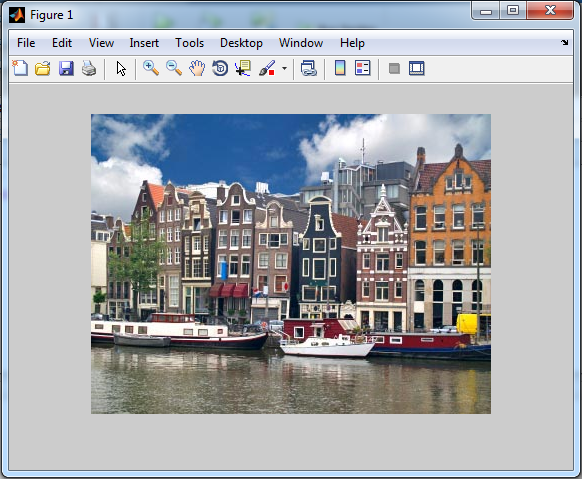
\includegraphics[scale=0.7]{src/ch7/holland_imshow.png}
\captionof{figure}{Bla bla}
\end{center}

La función \texttt{imshow} abre una nueva ventana (figure) y muestra la imagen que ha sido 
guardada con anterioridad  (ver figura 7.1). MATLAB dispone de otras funciones como 
\texttt{image} e \texttt{imagesc}  que también muestran en pantalla las imágenes, pero que suelen 
utilizarse más para la visualización en análisis de datos.

\section{Operaciones básicas con imágenes}

\subsection{Operaciones aritméticas}

Recuerde que una imagen en MATLAB se almacena como una matriz de mxnxp dimensiones, 
luego, es posible realizar operaciones aritméticas de suma, resta y multiplicación sobre 
ella como una matriz común, tal como se ha visto en Capítulo 2.

\subsubsection{Suma de un escalar}

Si sumamos una constante k a una matriz \textbf{A}, entonces cada elemento de \textbf{A} se incrementa en k 
unidades, lo cual se traduciría en un aumento del brillo en la imagen. Véase el ejemplo siguiente:

\begin{verbatim}
	A=imread('imag.jpg');
	k=50;
	A=A+k;
	imshow(A);
\end{verbatim}

\begin{center}
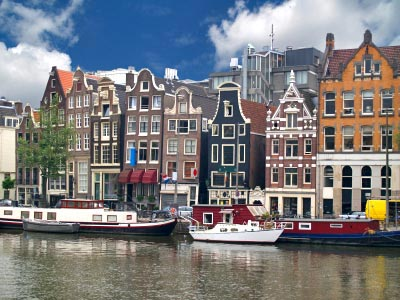
\includegraphics[scale=0.7]{src/ch7/holland_original.png}
\captionof{figure}{Imagen original}
\end{center}

\begin{center}
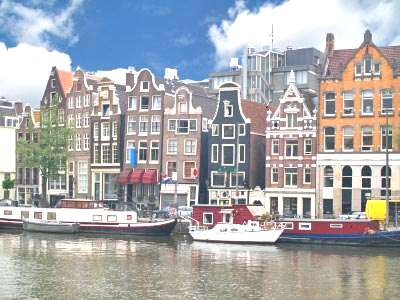
\includegraphics[scale=0.7]{src/ch7/holland_mas50.png}
\captionof{figure}{Imagen aumentada en 50 unidades}
\end{center}

La imagen 7.2 corresponde a la original y en la 7.3 se muestra lo que resulta de aumentar 
en 50 unidades cada uno de los pixeles que componen la imagen.

\subsubsection{Resta de un escalar}

Es evidente que la resta de un escalar es muy similar en interpretación a la suma vista 
anteriormente, solo que en este caso cada elemento de la matriz disminuye en un valor 
constante. Véase el ejemplo:

\begin{verbatim}
	A=imread('img.jpg');
	k=80;
	A=A-k;
	imshow(A);
\end{verbatim}

\begin{center}
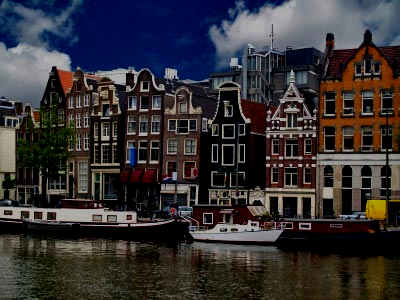
\includegraphics[scale=0.7]{src/ch7/holland_menos50.png}
\captionof{figure}{Imagen disminuida en 50 unidades}
\end{center}

\subsection{Conversión a escala de grises}

La escala de grises es una forma de representar imágenes digitales utilizando solamente variaciones 
de grises, desde negro a blanco.\\

En MATLAB se dispone de la función \texttt{rgb2gray} para convertir una imagen dada en el modelo de color RGB 
a una imagen en escala de grises.

\begin{verbatim}
X=imread('img.png');
XG=rgb2gray(X);
imshow(XG);
\end{verbatim}

\begin{center}
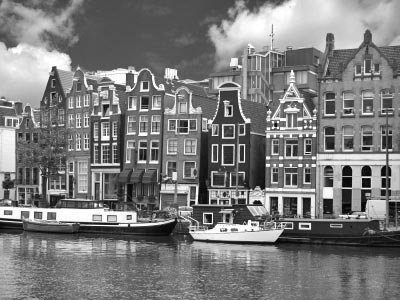
\includegraphics[scale=0.7]{src/ch7/holland_gris.png}
\captionof{figure}{Imagen en escala de grises}
\end{center}

\subsection{Binarización de una imagen}

\section{Segmentación de imágenes}

\subsection{Umbralización}

\subsection{Detección de bordes}

\section{Restauración y mejoramiento de imágenes}

\subsection{Removiendo ruido}
\chapter{Introducción a las GUIs MATLAB}

Una interfaz gráfica de usuario (GUI) es un elemento gráfico que contiene uno o más controles que están disponibles 
para interactuar con el usuario mediante un entorno visual sencillo, el cual permite la comunicación entre el usuario 
y el computador. Entre algunos de los componentes más comunes de una GUI creada en MATLAB se tienen menús, barras de 
herramientas, botones, menús desplegables, cajas de texto, entre otros.\\

En las interfaces gráficas creadas en MATLAB pueden aprovecharse todas las herramientas matemáticas y de ingeniería 
que proporciona MATLAB, permiten además la manipulación de archivos de datos, así como la interacción con otras GUIs 
y mostrar datos mediante tablas y gráficas de gran calidad.\\

Generalmente las GUIs son programadas para que respondan a la manipulación del usuario con una acción específica. 
Los controles gráficos que componen una GUI están relacionados con una rutina de programación, llamada callbacks 
en el entorno MATLAB, que se ejecuta cuando sucede  un determinado evento, que puede ser la entrada de caracteres 
mediante el teclado, el clic de un botón del mouse, o situarse sobre un objeto.

\section{Elemento figure}

En MATLAB cada interfaz gráfica está creada sobre un objeto figure, en este elemento se añaden 
todos los controles gráficos que componen la GUI. La forma más simple de definir un objeto 
figure se ejemplifica enseguida:

\begin{verbatim}
	hFig = figure;
\end{verbatim}

Donde \texttt{hFig} es el handle del elemento figure.\\

Es muy común que al momento de definir o crear un objeto figure, se especifiquen algunas 
de sus propiedades con la sintaxis siguiente:

\begin{verbatim}
	hFig = figure('Propiedad ', 'Valor ',...);
\end{verbatim}

A continuación se muestra un ejemplo característico:

\begin{verbatim}
	hFig = figure('NumberTitle','off',...
	              'MenuBar','None',...
	              'Name','Figure Ejemplo',...
	              'Position',[200 200 300 300]);
\end{verbatim}

Las propiedades más comunes de un elemento figure se muestran en la tabla siguiente:

\begin{table}[h!]
\centering
{\rowcolors{1}{}{gray!20}
\begin{tabular}{p{3cm} p{12cm}}
\rowcolor{LightBlue2} \textbf{Propiedad} & \textbf{Descripción} \\
\texttt{Color} & Establece el color de figure. El valor puede establecerse mediante 
un vector de tres elementos en formato RGB \\

\texttt{MenuBar} & Oculta o muestra la barra de menús estándar de MATLAB \\

\texttt{Name} & Título mostrado en la ventana de la figura. El valor especificado es una cadena de caracteres \\

\texttt{NumberTitle} & Determina si la numeración de los elementos figure creada automáticamente por MATLAB será visible. El valor por defecto es on, para ocultar deberá especificarse off. \\

\texttt{Position} & Especifica el tamaño de la GUI y la posición relativa a la esquina inferior
izquierda de la pantalla. El valor se establece mediante un vector de cuatro
elementos cuya estructura es la siguiente: [Distancia de la
izquierda, Distancia de la parte inferior, Ancho, Alto]; \\

\texttt{Resize} & Determina si puede modificarse el tamaño de la GUI utilizando el mouse. Los
valores aceptados son: off y on, siendo este último el valor por defecto. \\

\texttt{Toolbar} & Muestra o borra el menú de herramientas del objeto figure. \\

\texttt{Units} & Unidad de medida que se utilizará para interpretar el vector de la propiedad
position. Los valores disponibles son: centimeters, characters,
inches, normalized, point y pixels. Siendo este último el valor por defecto. \\

\texttt{Visible} & Establece si la GUI es visible. Valores: on y off. \\

\end{tabular}
\caption{Propiedades de \texttt{figure}}
\end{table}



\section{Controles gráficos (uicontrol)}

Los controles gráficos son creados mediante la función uicontrol, cuya estructura general se muestra:

\begin{verbatim}
	hCont = uicontrol('Style', 'tipo de control',...
	                  'Propiedad', 'Valor');
\end{verbatim}

La propiedad \texttt{style} define el tipo de control gráfico
\chapter{Programación orientada a objetos}

\section{Conceptos básicos de la POO}

La programación orientada a objetos (POO) es un paradigma de programación que utiliza 
objetos como parte esencial de sus interacciones, para el desarrollo de aplicaciones y 
soluciones tecnológicas. La POO está soportada por técnicas de programación tales como 
la herencia, el polimorfismo, el encapsulamiento, entre otras, cada una de ellas 
proporciona herramientas que han permitido la proliferación de este modelo de programación 
en las últimas décadas. Actualmente existen una variedad de lenguajes que soportan la POO, 
siendo los más conocidos C++, Java y C#.\\

El soporte \textit{moderno} de MATLAB para la POO es relativamente nuevo, siendo 
introducido a partir de la versión 7.6 (R2008a) con notables carencias respecto a los 
lenguajes de referencia en ese aspecto, pero evidentemente la mejora desde entonces 
ha sido considerable.\\

\begin{quote}
Con soporte \textit{moderno} se hace alusión a la notación actual que se utiliza en la definición 
de clases, por ejemplo \texttt{classdef} para crear una clase. Puesto que antes de la implementación 
de esta notación, existía la posibilidad de programar orientado a objetos haciendo uso de algunos 
\textit{artilugios}, como el colocar la clase (definida mediante una función que hacía lo de un 
\textit{constructor} de la clase) y sus métodos dentro de una carpeta cuyo nombre debería ser 
el de la clase misma anteponiéndole un arroba (@). 
\end{quote}

\subsection{Clases y objetos}

Una clase es una definición de las propiedades y/o características de un determinado tipo 
de objetos, es decir, un modelo particular que sirve para crear objetos bajo esas 
mismas especificaciones.\\ 

Un objeto es la representación concreta derivada de una clase que está provisto de 
atributos y métodos, o en términos más formales: un objeto es la instancia de una clase.\\

A manera de ejemplo y un contexto más apegado a la realidad, consideremos a los perros 
como una determinada clase, es sencillo hacernos la idea de cómo es un perro y cuáles 
son sus características y apariencia general; luego, el perro que tenemos en casa 
(en caso de que así sea) es una instancia de esa clase o un objeto de la clase perro, 
con características más particulares  pero que no les excluyen de ser un perro.\\

\subsection{Atributos}

Los atributos son las propiedades asociadas a una clase de objetos. Siguiendo con el 
ejemplo de los perros, estos tienen atributos como el tamaño, color, raza, temperamento, etc. 
Es común en la POO diferenciar entre dos tipos de atributos acorde a su accesibilidad: 
los privados y los públicos. Los privados son atributos disponibles solo dentro de la 
definición de la clase, en cambio los públicos son accesibles desde cualquier otra clase 
o fichero de instrucciones.

\subsection{Métodos}

Los métodos de una clase de objetos son algoritmos o bloques de programación que 
determinan el comportamiento de un objeto. Por lo general los métodos se usan para 
modificar los atributos de un objeto o bien generar un nuevo evento. En MATLAB los 
métodos son definidos mediante funciones.

\subsection{Eventos}

Un evento es la \textit{reacción} que tiene un objeto resultante de la interacción con 
el usuario o bien mediante la ejecución de los métodos.

\section{Definiendo clases en MATLAB}

Las clases son el \textit{alma} de la POO, y suelen definirse en ficheros únicos. En 
MATLAB pueden crearse utilizando un fichero *.m ordinario y colocando en este la 
sintaxis para la definición de una clase, la cual se muestra enseguida:

\begin{verbatim}
	classdef nombreClase
	    % Descripción de la clase
	    
	    properties
	        % Atributos
	    end
	    
	    methods
	        % Métodos
	    end
	    
	end
\end{verbatim}

En la mayoría de los lenguajes que soportan POO se utiliza la palabra clave class 
para definir una clase, pero en MATLAB class se utiliza para identificar el tipo 
o clase de una variable u objeto, y en cambio se utiliza classdef para definir 
una clase. Los atributos de una clase se definen en un bloque properties-end, y 
pueden simplemente ser declarados sin asignación de valores. Los métodos de la 
clase se especifican dentro de un bloque methods-end, incluyendo al constructor 
de la clase.

\subsection{El constructor de la clase}

El constructor de una clase es parte esencial de la misma y en este se definen 
los argumentos o parámetros formales necesarios para crear un objeto de la clase, 
de ahí su importancia. En MATLAB el constructor se considera, de manera no estricta, 
un método y por tanto se define dentro del bloque correspondiente a los métodos. 
Así pues, incluyendo al constructor la definición de una clase sería algo similar a:

\begin{verbatim}
	classdef nombreClase
	    % Descripción de la clase
	    
	    properties
	        % Atributos
	    end
	    
	    methods
	        function obj = nombreClase(args)
	           % Constructor de la clase 
	        end
	        % ...
	        % Métodos
	        % ...
	    end
	    
	end
\end{verbatim}

En lo anterior obj es, dentro la definición de la clase, una referencia al objeto 
instanciado y es obligatorio el colocarlo como \textit{valor de salida} (en la terminología 
de funciones); claro que el identificador \texttt{obj} puede cambiarlo por cualesquiera 
otro de su comodidad (\texttt{this} o \texttt{self} podrían ser buenas opciones, claro, 
mucho influye el hecho de haber programado en otro lenguaje de POO en este tipo de 
\textit{adopciones} de estilo). Tal como se ejemplifica, el nombre de la función que funge 
como constructor debe ser el mismo que el de la clase, además deben especificarse los 
argumentos que se utilizarán para crear un objeto.

\section{La clase Persona, una primera aproximación}

En la sección anterior hemos visto la sintaxis para definir una clase, pero como casi 
todo siempre es mejor asociar un concepto teórico con un ejemplo concreto. Para tal fin 
crearemos la clase Persona, de naturaleza muy sencilla pero significativa.\\

En principio vamos a definir las propiedades o atributos que habrán de caracterizar a un 
objeto de la clase Persona, así pues, dada la simplicidad del caso solamente utilizaremos 
el nombre y la edad para \textit{construir} un objeto de esta clase. Por ahora no definiremos 
método alguno, solamente el constructor de la clase. Véase la definición resultante:

\begin{verbatim}
	classdef Persona
	    % Persona
	    %
	    % Ejemplo :
	    %           p1 = Persona('Jorge',22);
	    %           p2 = Persona('Anna',28);          
	    %
	    
	    properties % Atributos de la clase
	        nombre;
	        edad;
	    end
	    
	    methods
	        function obj = Persona(nombre,edad) % Constructor
	            obj.edad=edad;
	            obj.nombre=nombre;
	        end
	    end
	    
	end
\end{verbatim}

Para \textit{testear} una clase podemos crear un script en donde colocar las instrucciones 
necesarias para crear un objeto de la misma. No obstante, por ahora haremos esto en 
la ventana de comandos de la siguiente manera:

\begin{verbatim}
	>> p = Persona('Ana',25);
	>> whos
	  Name      Size            Bytes  Class      Attributes
	  p         1x1               118  Persona        
\end{verbatim}
\chapter{Recomendaciones generales}

\section{Escribiendo código legible}

La legibilidad cuenta, claro que sí. Una frase de Abelson y Sussman, en el libro Estructura e interpretación de 
Programas de Computadora, lo resume de forma notable: \textit{Los programas deben escribirse para que los lean las 
personas y solo de forma circunstancial para que los ejecuten las máquinas.}\\

De modo que cuando se escribe código, en cualquier lenguaje de programación, es importante estructurar 
los programas de una forma que resulte entendible para cualquier individuo. Entonces, se deben desarrollar 
lineas de código pensando en que en algún momento alguien más tratará de entenderlo (sí, aun cuando esto sea 
poco probable).\\

A continuación se listan algunas recomendaciones básicas para estructurar un programa:

\subsection{Nombres de variables autodescriptivos}

Siempre que sea posible es preferible utilizar nombres de variables autodescriptivos, aún cuando estos resulten 
un poco extensos. La ganancia en legibilidad lo compensa todo, por ejemplo, es preferible tener:

\begin{verbatim}
	fuerza = 10;
	area = 20;
	presion = fuerza/area;
\end{verbatim}

a simplemente colocar:
	
\begin{verbatim}
	f = 10;
	a = 20;
	p = f/a;
\end{verbatim}

\subsection{Indentación del código}

Una buena indentación del código permite distinguir los diversos bloques de programación. Actualmente el editor
de MATLAB proporciona herramientas que facilitan esta tarea, simplemente seleccionando el código y presionando 
Ctrl + I para un \textit{indentado inteligente}. Note las diferencias entre los códigos siguientes:

\begin{verbatim}
	k = 1;
	while true
	if rem(k,2)==0
	disp('Par');
	else
	disp('Impar');
	end
	k = k + 1;
	end
\end{verbatim}

\begin{verbatim}
	k = 1;
	while true
	    if rem(k,2)==0
	        disp('Par');
	    else
	        disp('Impar');
	    end
	    k = k + 1;
	end
\end{verbatim}



\subsection{Documentación del código}

\subsection{Espacios}


\section{Optimizando el código}


\subsection{Pre-asignación (pre-allocation)}

Una de las grandes ¿ventajas? de MATLAB es su \textit{tipado dinámico}

\subsection{Vectorización}

\printindex

\end{document}